\documentclass[11pt, a4paper]{article}

% ── Encoding & fonts ──────────────────────────────────────────────────────────
\usepackage[utf8]{inputenc}
\usepackage[T1]{fontenc}
\usepackage{lmodern}
\usepackage{microtype}

% ── Mathematics ───────────────────────────────────────────────────────────────
\usepackage{amsmath, amssymb, amsthm}
\usepackage{mathtools}          % extends amsmath
\usepackage{bbm}                % \mathbbm{1} indicator function


% ── Layout ────────────────────────────────────────────────────────────────────
\usepackage[margin=1.2in]{geometry}
\usepackage{setspace}
\onehalfspacing

% ── Figures & colour ──────────────────────────────────────────────────────────
\usepackage{graphicx}
\usepackage{float}
\usepackage[dvipsnames]{xcolor}

\usepackage{caption}
\captionsetup{
    font=small,        % smaller font than body text
    labelfont=bf,      % "Figure 1" in bold
    margin=1cm,        % indent the caption from the edges
    justification=centerlast  % last line centred, rest justified
}

\usepackage{subcaption} % in preamble

% ── Hyperlinks ────────────────────────────────────────────────────────────────
\usepackage[
  colorlinks = true,
  linkcolor  = MidnightBlue,
  citecolor  = MidnightBlue,
  urlcolor   = MidnightBlue
]{hyperref}

% ── References ────────────────────────────────────────────────────────────────
\usepackage[
  backend  = biber,
  style    = alphabetic,
  sorting  = nyt
]{biblatex}
\addbibresource{refs.bib}

% ── Theorem environments ──────────────────────────────────────────────────────
\theoremstyle{plain}
\newtheorem{theorem}{Theorem}[section]
\newtheorem{lemma}[theorem]{Lemma}
\newtheorem{proposition}[theorem]{Proposition}
\newtheorem{corollary}[theorem]{Corollary}

\theoremstyle{definition}
\newtheorem{definition}[theorem]{Definition}
\newtheorem{example}[theorem]{Example}

\theoremstyle{remark}
\newtheorem{remark}[theorem]{Remark}

% A plain-language aside: the same point again without the machinery.
\newenvironment{plainly}
  {\par\smallskip\begin{quote}\small\noindent
   \textcolor{MidnightBlue}{\textbf{In plain terms.}}\enspace\ignorespaces}
  {\end{quote}\smallskip}

% ── Operators & shorthands ────────────────────────────────────────────────────
\DeclareMathOperator{\diam}{diam}
\newcommand{\R}{\mathbb{R}}
\newcommand{\N}{\mathbb{N}}
\newcommand{\Hm}[1]{\mathcal{H}^{#1}}   % Hausdorff measure
\newcommand{\Hd}{\dim_{\mathcal{H}}}     % Hausdorff dimension
\newcommand{\Bd}{\dim_{\mathrm{box}}}    % box-counting dimension
\newcommand{\eps}{\varepsilon}
\newcommand{\Z}{\mathbb{Z}}

% ─────────────────────────────────────────────────────────────────────────────

\title{%
  \textbf{Fractal Dimension: Theory and Computation}\\[0.4em]
  \large Box-Counting Estimation via Hilbert Curve Analysis
}
\author{ME}
\date{\today}

\begin{document}

\maketitle
\tableofcontents
\newpage

% ─────────────────────────────────────────────────────────────────────────────
\section{Introduction}
\label{sec:intro}
% ─────────────────────────────────────────────────────────────────────────────

This entire paper is basically based on \cite{falconer2003}. This is just what I found when I wanted to look into this area.\\
Classical dimension is usually viewed at as an integer e.g. a square is 2D. However, is there a way to consider dimension in another manner? Geometric objects in nature (e.g. coastlines, trees, etc.) exhibit self similarity at all scales and resist this classification. How do we measure the ``size'' for such a set? Is there a scaling property associated with dimension?\\
This short write-up develops the measure theory needed to understand said property (Hausdorff measure and dimension), and introduces ways to compute measure (through the box-counting dimension). We use the Hilbert curve as a case study in which we can analytically derive the dimension and computationally estimate it.
\newpage
\section{Measure Theory}

\noindent\textit{The material in this section is standard and follows 
the presentation in \cite{menegaki2026}.}\\\\
First to define measure theory (I didn't take Lebesgue so I will be using the above notes...)\\\\
A measure is a way to assign a ``size'' to subsets of a set X. Let $\mathcal{F}$ be a $\sigma$-algebra on X.\\
\begin{definition} (Measure). Let (\textit{X}, $\mathcal{F}$) be a measurable space. A measure on (X, $\mathcal{F}$) is a function $\mu : \mathcal{F} \rightarrow [0, \infty]$ satisfying:
\begin{enumerate}
\item $\mu(\emptyset) = 0$
\item \textbf{Countable additivity:} if $A_1, A_2, \ldots \in \mathcal{F}$ are 
    pairwise disjoint, then
    \[
      \mu\!\left(\bigsqcup_{i=1}^{\infty} A_i\right) = \sum_{i=1}^{\infty} \mu(A_i)
    \]
\end{enumerate}
The triple $(X, \mathcal{F}, \mu)$ is called a \textbf{measure space}.
\end{definition}
\vspace{2pt}\begin{proposition}[Basic properties]
  Let $(X, \mathcal{F}, \mu)$ be a measure space.
  \begin{enumerate}
    \item \textbf{Monotonicity}: \[A \subseteq B \Rightarrow \mu(A) \leq \mu(B)\]
    \item \textbf{Countable subadditivity}: 
    \[\mu\!\left(\bigcup_{i=1}^{\infty} A_i\right) \leq \sum_{i=1}^{\infty} \mu(A_i)\]
    \item \textbf{Continuity from below}: if $A_1 \subseteq A_2 \subseteq \cdots$ then
    \[
      \mu\!\left(\bigcup_{i=1}^{\infty} A_i\right) = \lim_{i \to \infty} \mu(A_i)
    \]
    \item \textbf{Continuity from above}: if $A_1 \supseteq A_2 \supseteq \cdots$ 
    and $\mu(A_1) < \infty$ then
    \[
      \mu\!\left(\bigcap_{i=1}^{\infty} A_i\right) = \lim_{i \to \infty} \mu(A_i)
    \]
  \end{enumerate}
\end{proposition}

The canonical example is the \textbf{Lebesgue measure} $\lambda^n$ on 
$(\R^n, \mathcal{B}(\R^n))$, where $\mathcal{B}(\R^n)$ is the Borel $\sigma$-algebra 
--- the smallest $\sigma$-algebra containing all open sets. Lebesgue measure assigns 
to each box $[a_1, b_1] \times \cdots \times [a_n, b_n]$ its volume 
$(b_1 - a_1) \cdots (b_n - a_n)$, and extends uniquely to all Borel sets. It 
formalises the intuitive notions of length, area, and volume.

The inadequacy of Lebesgue measure for fractal geometry is immediate: a curve 
$\gamma \subset \R^2$ has $\lambda^2(\gamma) = 0$ (zero area) but $\lambda^1(\gamma)$ 
may be infinite (infinite length). Neither gives useful information about the 
``size'' of $\gamma$. What is needed is a family of measures parametrised by a 
continuous exponent $s \geq 0$.

To construct such a family, we need the notion of an outer measure, which is 
slightly weaker than a measure --- it is defined on \emph{all} subsets of $X$, 
not just measurable ones, and only requires subadditivity rather than full 
additivity.

\begin{definition}[Outer measure]
  A function $\mu^* : 2^X \to [0, \infty]$ is an \textbf{outer measure} on $X$ if:
  \begin{enumerate}
    \item $\mu^*(\emptyset) = 0$
    \item \textbf{Monotonicity}: $A \subseteq B \Rightarrow \mu^*(A) \leq \mu^*(B)$
    \item \textbf{Countable subadditivity}:
    \[
      \mu^*\!\left(\bigcup_{i=1}^{\infty} A_i\right) 
      \leq \sum_{i=1}^{\infty} \mu^*(A_i)
    \]
  \end{enumerate}
\end{definition}

The relationship between outer measures and measures is given by the
Hahn-Carath\'{e}odory extension theorem: given an outer measure $\mu^*$ on $X$, the collection
\[
  \Sigma = \{A \subseteq X : \mu^*(B) = \mu^*(B \cap A) + \mu^*(B \setminus A) 
  \text{ for all } B \subseteq X\}
\]
is a $\sigma$-algebra, and $\mu^*|_{\Sigma}$ is a measure. Sets in 
$\Sigma$ are called \textbf{$\mu^*$-measurable}. In particular, all Borel sets  
are $\mu^*$-measurable whenever $\mu^*$ is constructed from a Borel-compatible 
pre-measure --- which will be the case for Hausdorff measure.

The standard way to construct an outer measure is via coverings. If 
$\mathcal{K} \subseteq 2^X$ covers $X$ (with $\emptyset \in \mathcal{K}$) and 
$\tilde{\mu} : \mathcal{K} \to [0, \infty]$ assigns sizes to sets in $\mathcal{K}$ 
with $\tilde{\mu}(\emptyset) = 0$, then
\[
  \mu^*(A) = \inf\left\{
    \sum_{i=1}^{\infty} \tilde{\mu}(K_i) 
    \;\middle|\; 
    K_i \in \mathcal{K},\ A \subseteq \bigcup_{i=1}^{\infty} K_i
  \right\}
\]
defines an outer measure on $X$. This is precisely the construction used to 
define Hausdorff measure --- with $\mathcal{K}$ being all subsets of diameter 
at most $\delta$, and $\tilde{\mu}(U) = |U|^s$.
% ─────────────────────────────────────────────────────────────────────────────
\newpage
\section{Hausdorff Measure}
The material in sections 3 and 4 follows \cite{falconer2003}.
\subsection{Definition} Let ($X$, $d$) denote  a metric space, $S \subseteq X$ a Borel set. \\For a set $U \subseteq X$, write $|U| := $ diam($U$) $= sup_{x,y\in U}d(x, y)$
\begin{definition}
    Let $s \geq 0,$ and $\delta > 0$. Define \[
    \Hm{s}_\delta(S) = \inf\left\{
      \sum_{i=1}^{\infty} |U_i|^s 
      \;\middle|\; 
      S \subseteq \bigcup_{i=1}^{\infty} U_i,\ |U_i| \leq \delta
    \right\}
    \]
    This is the infimum over all countable covers of S by sets of diameter at most $\delta$.
\end{definition}
\noindent As $\delta \rightarrow 0$, we allow fewer and fewer covers, so $\Hm{s}_\delta(S)$ is non-decreasing in $1/\delta$. The limit \[
\Hm{s}(S) = \lim\limits_{\delta\rightarrow 0}\Hm{s}_{\delta}(S)\in [0, \infty]
\]
is the $s$-dimensional Hausdorff measure of $S$. This is possibly $+\infty$.\\
$\Hm{s}$ is an outer measure on $X$, and its restriction to the Borel $\sigma$-algebra is a measure. 

\subsection{Phase Transition}
Observe that $\Hm{s}(S)$ exhibits a phase transition in $s$:
\begin{theorem}
    If $\Hm{s}(S) < \infty$ for some $s$, then $\Hm{t}(S) = 0$ for all $t > s$.
\end{theorem}
\begin{proof}
    Suppose $\Hm{s}(S) < \infty$. For any cover $\{U_i\}$ with $|U_i| \leq \delta$. For $t>s$:\[
    \Sigma|U_i|^t=\Sigma|U_i|^{t-s}\cdot|U_i|^s\leq\delta^{t-s}\Sigma|U_i|^s
    \]
    Taking the infimum over all covers gives \[\Hm{t}_\delta(S) \leq \delta^{t-s}\cdot\Hm{s}_\delta(S)\leq\delta^{t-s}\cdot\Hm{s}(S)\] where the second inequality holds since $\Hm{s}_\delta(S)$ is non-decreasing in $1/\delta$.\\
    Now let $\delta\rightarrow0$, $t-s>0$, and $\Hm{s}(S) < \infty$ is a fixed finite constant. So the right hand side goes to 0, hence $\Hm{t}(S)=0$.
\end{proof}
\begin{corollary}
There exists a unique value $d\in[0, \infty]$ such that\[
\Hm{s}(S) = \begin{cases} 
\text{$\infty$}&\text{$s < d$}\\
\text{$0$}&\text{$s > d$}
\end{cases}
\]
At $s=d$, the measure $\Hm{d}(S)$ may take any value in $[0, +\infty]$.
\end{corollary}
\newpage
\section{Hausdorff Dimension}
\begin{definition}
    (Hausdorff Dimension). The \textbf{Hausdorff Dimension} of S is the critical exponent\[
    \Hd(S) = \text{inf}\{s\geq0:\Hm{s}(S)=0\} = \text{sup}\{s\geq0:\Hm{s}(S)=+\infty\}
    \]
\end{definition}
\noindent This is the ``true'' dimension of a fractal.
\subsection{Basic Properties}
\begin{proposition}[Basic properties]
Hausdorff dimension satisfies the following:
\begin{enumerate}
    \item \textbf{Monotonicity}: $A \subseteq B \implies \Hd(A) \leq \Hd(B)$
    \item \textbf{Countable stability}: $\Hd(\cup_{i=1}^{\infty}A_i)=\sup_i\Hd(A_i)$
    \item \textbf{Countable sets}: if $S$ is countable, $\Hd(S) = 0$.
    \item \textbf{Smooth manifolds
\footnote{A smooth $k$-dimensional manifold is just a set that locally looks like $\mathbb{R}^k$}}: if $M \subset \mathbb{R}^n$ is a smooth k-dimensional submanifold, then $\Hd(M) = k$.
  \end{enumerate}
\end{proposition}
\vspace{5pt}\noindent The following proposition is a useful tool we'll need later down the line:
\begin{proposition}{(Lipschitz invariance).}
    Let $f: A\rightarrow B$ be Lipschitz with constant C. Then $\Hd(f(A))\leq\Hd(A)$. In particular, bi-Lipschitz maps preserve Hausdorff dimensions.
\end{proposition}
\begin{proof}
    If $\{U_i\}$ covers A with $\Sigma|U_i|^s<\infty$, then $\{f(U_i)\}$ covers $f(A)$ with $|f(U_i)|\leq C|U_i|$ (by Lipschitz), so $\Sigma|f(U_i)|^s\leq C^s\Sigma|U_i|^s<\infty$ Hence $\Hm{s}(f(A))\leq C^s\Hm{s}(A)$, and the dimension inequality follows.
\end{proof}
\newpage
\section{Box-counting Dimension}
\subsection{Definition}
\label{sec:boxdef}
A.K.A Minkowski–Bouligand dimension.\\
We need a way to be able to effectively compute the dimension of a fractal (i.e. the Hausdorff dimension). A perhaps easy way to do this is to cover said shape with boxes of size $\eps$ and count them. We check to see how the number of boxes hitting the shape $N(\eps)$ changes w.r.t the length $\eps$. We use the following formula: 
\[
\Bd(S) := \lim\limits_{\eps\rightarrow0}\frac{\log N(\eps)}{\log (1/\eps)} = -\lim\limits_{\eps\rightarrow0}\frac{\log N(\eps)}{\log (\eps)}
\]
This is roughly the dimension $d$ such that $N(\eps) \approx C\eps^{-d}$.\\
Note that this is a limit taken on the set itself. Evaluated on a picture of the set (which is all a computer ever has) it misbehaves, and \S\ref{sec:rolloff} measures how badly.\\
Intuitively, we choose this to represent the dimension because a $d$-dimensional box of side $\eps$ has a ``$d$-dimensional volume'' $\eps^d$. So we end up with some $N(\eps) \approx \frac{V}{\eps^{d}} = C\eps^{-d}$. We want to find a $d$ for a fractal i.e. finding the $d$ such that the same scaling property holds.

\subsection{Relationship to Hausdorff dimension}
\begin{proposition}
    For any bounded $S\subseteq\mathbb{R}^n$ whose box dimension exists,
    $\Hd(S)\leq\Bd(S)$.
\end{proposition}
\begin{proof}
    Let $d>\Bd(S)$ and pick $s$ with $\Bd(S)<s<d$. 
    Since $\log N(\eps)/\log(1/\eps)\to\Bd(S)<s$, we have $N(\eps)\leq\eps^{-s}$ 
    for all sufficiently small $\eps$. Covering $S$ with these $N(\eps)$ boxes, each of diameter $\eps\sqrt{n}$,
    \[
    \Hm{d}_{\eps\sqrt{n}}(S)\leq N(\eps)\,(\eps\sqrt{n})^d
    \leq(\sqrt{n})^d\,\eps^{\,d-s}\rightarrow0
    \]
    as $\eps\rightarrow0$, since $d-s>0$. Hence $\Hm{d}(S)=0$, so
    $\Hd(S)\leq d$. Since $d>\Bd(S)$ was arbitrary, $\Hd(S)\leq\Bd(S)$.
\end{proof}
\noindent This is a very useful property as will be shown in the next few chapters. With this we now have a best upper bound for calculting the Hausdorff dimension. The equality actually holds on ``well-behaved'' fractals which is exactly what we need. 
\newpage
\section{Self-similar sets and Moran's theorem}
This section explores \cite{fernandezmartinez2016moran}.
\subsection{Iterated Function Systems}
\begin{definition}{(IFS and attractor).}
    An \textbf{iterated function system} (IFS) is a finite collection of contractions\footnote{A contraction $f$ is a function such that $d(f(x), f(y))\leq\alpha\cdot d(x,y)$, where $\alpha\in[0,1)$.} $\{f_1,...,f_N\}$ on a complete\footnote{A complete metric space is one such that every Cauchy sequence converges.} metric space $(X, d)$, where each $f_i$ has Lipschitz constant $r_i\in(0,1)$. The map $F(K)=\cup_{i=1}^Nf_i(K)$ on the space of compact\footnote{Compact sets are closed and bounded.} subsets of $X$ (using the Hausdorff metric - $d_H(A, B) = \max(\sup_{a\in A}d(a, B), \sup_{b\in B}d(b, A))$) is itself a contraction, so by the Banach fixed-point theorem there exists a unique compact \textbf{attractor} $K\subseteq X$ such that:
    \[
    K = \bigcup\limits_{i=1}^Nf_i(K)
    \]
\end{definition}
\begin{definition}{(Open set condition).}
    The IFS ${f_1,...,f_N}$ satisfies the \textbf{open set condition} (OSC) if there exists a non-empty bounded open set $V\subseteq X$ such that:
    \[
    \bigcup\limits_{i=1}^Nf_i(V)\subseteq V, \quad f_i(V)\cap f_j(V)=\emptyset \;\;\text{for}\;\; i\neq j
    \]
\end{definition}
This ensures the pieces of K do not overlap in a measure-theoretically significant way, which is necessary for the dimension formula to hold. Basically, any overlap would cause the dimension estimate to corrupt.

\subsection{Moran's theorem}
\begin{theorem}{(Moran, 1946).}
    Let $\{f_1,...f_N\}$ be an IFS of similarities on $\mathbb{R}^n$ with contraction ratios $r_1,...r_N\in (0,1)$, satisfying the OSC. Let $K$ be its attractor. Then
    \[
    \Hd(K)=\Bd(K)=s\text{,}
    \]
    where $s$ is the unique solution to the \textbf{Moran equation}
    \[
    \sum\limits_{i=1}^Nr_i^s=1.
    \]
\end{theorem}
Uniqueness of $s$ follows from the fact that $\varphi(s)=\Sigma_ir_i^s$ is strictly decreasing in $s$, with $\varphi(0)=N>1$ and $\varphi(\infty)=0$.\\
For a uniform IFS ($\forall i,\; r_i=r\in (0,1)$), the Moran equation gives $Nr^s=1$, hence $s=\log N/\log(1/r)$, which is the similarity dimension. A uniform IFS applies to all of your nice looking fractals. A non-uniform IFS (e.g. coastline) would have to have a numerical method of solving for this such as bisection or Newton's method.
\subsection{Examples}
\begin{example}{(Cantor set).}
    There are two similarities on $[0, 1]$, each with ratio $r=1/3$. We know this since at each iteration each line segment is replaced by 2 line segments, each a third of the length of the original. By Moran's theorem: $2\cdot(1/3)^s=1$, so $s=\log2/\log3\approx0.63092975$
\end{example}
\begin{figure}[h]
    \centering
    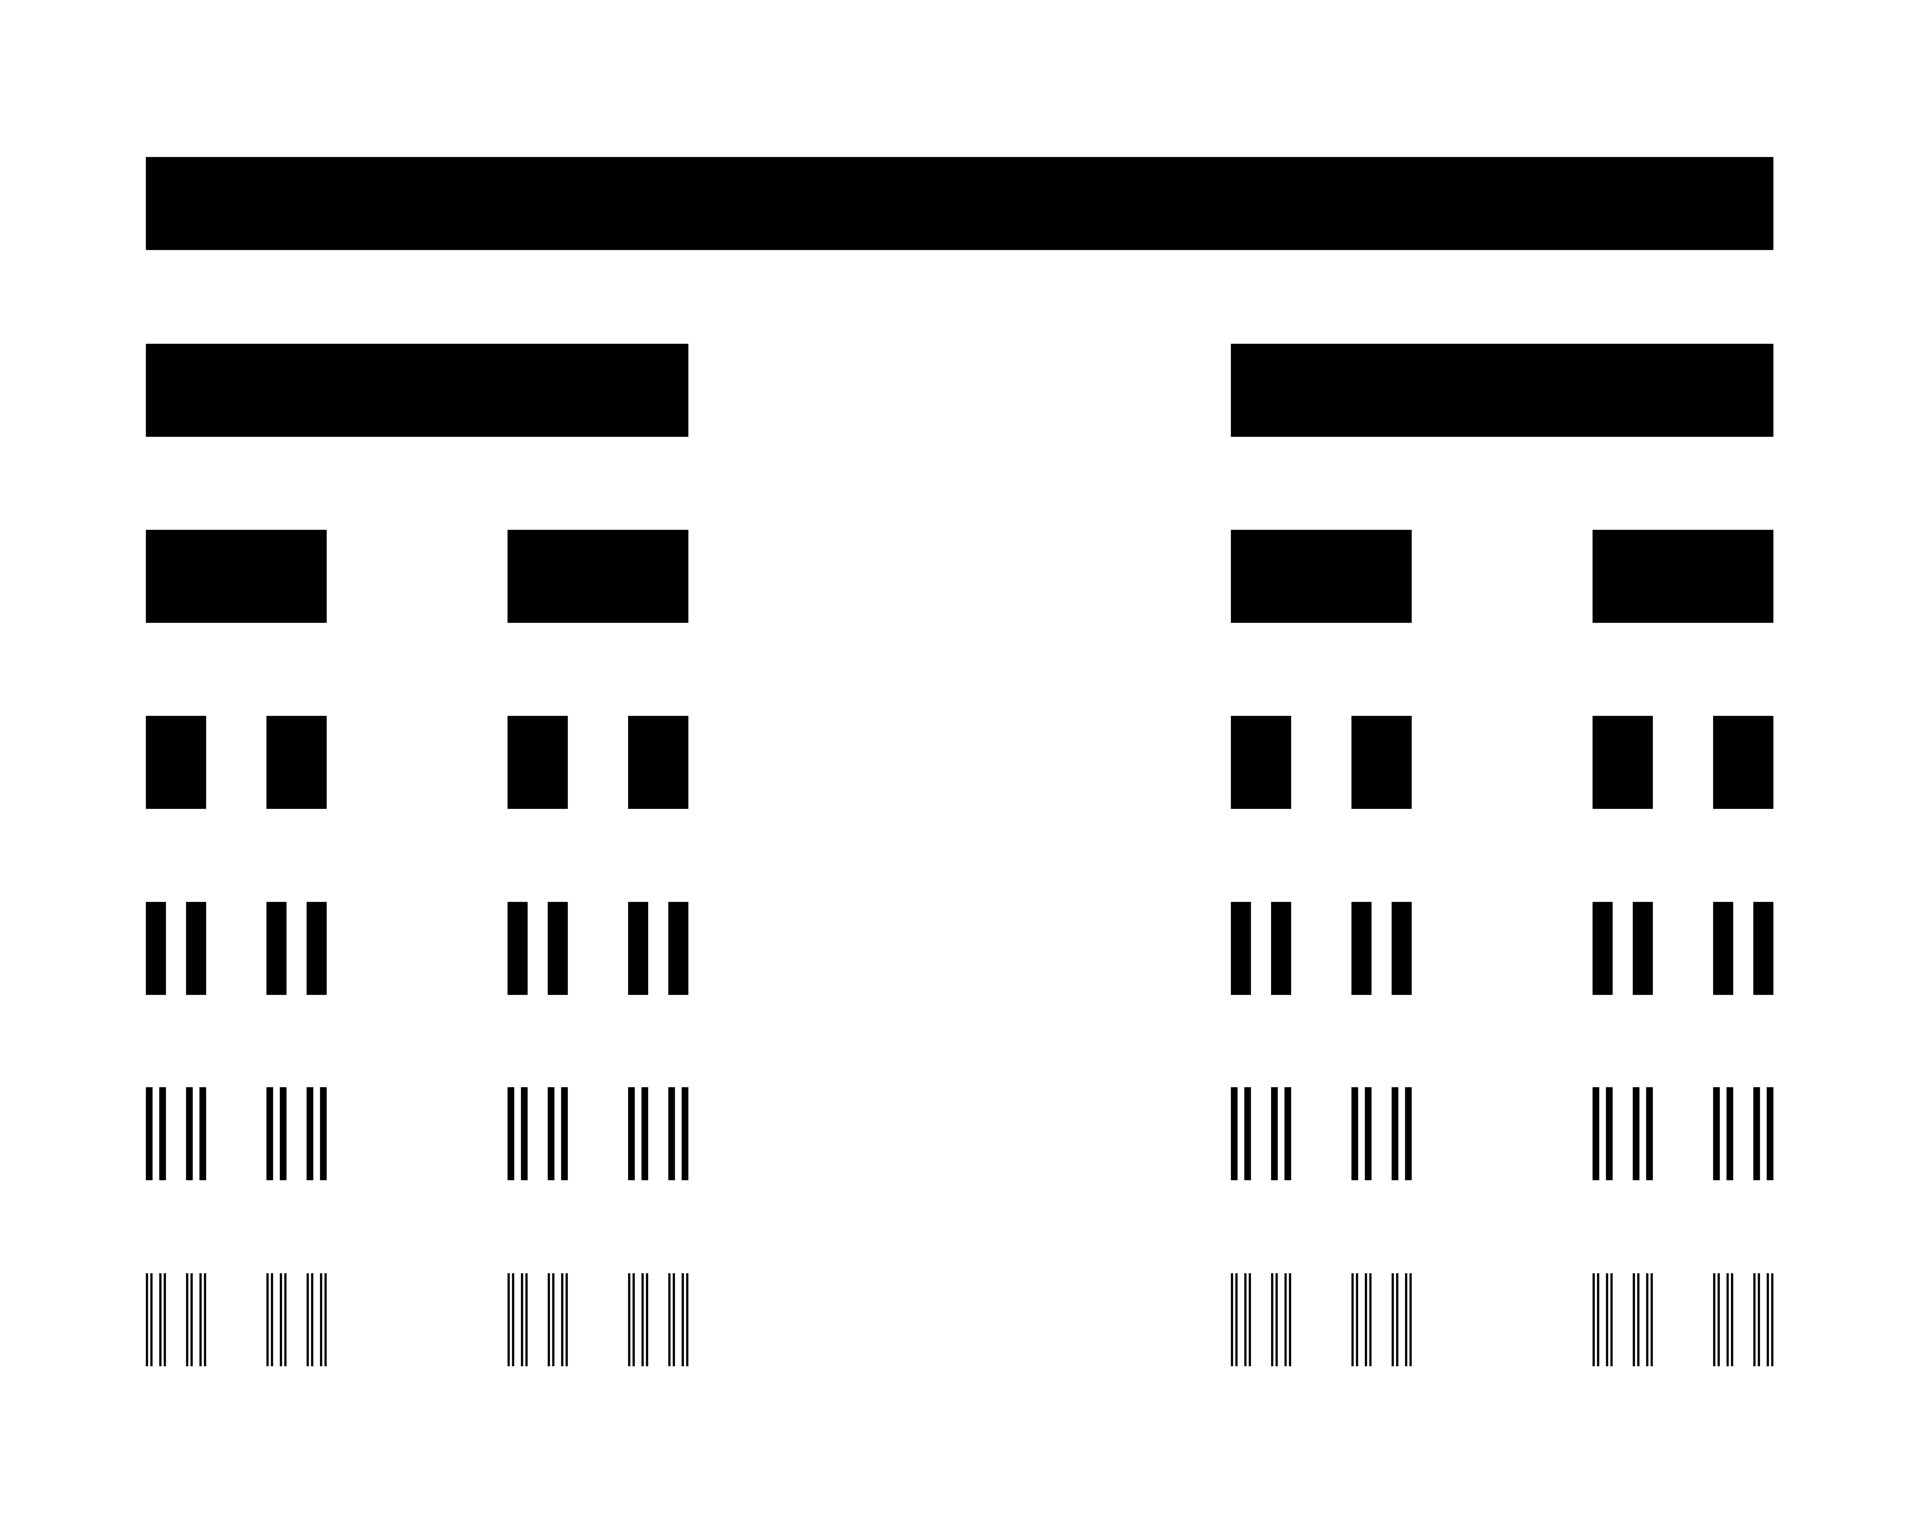
\includegraphics[width=0.5\textwidth]{images/Cantor.png}
    \caption{Cantor set construction (takes all values that aren't removed). \cite{img:cantor}}
    \label{fig:cantor}
\end{figure}
\begin{example}{(Serpi\'{n}ski triangle).}
    There are three similarities each with ratio $r=1/2$. By Moran's theorem: $3\cdot(1/2)^s=1$, so $s=\log3/\log2\approx1.58496250$
\end{example}
\begin{figure}[h]
    \centering
    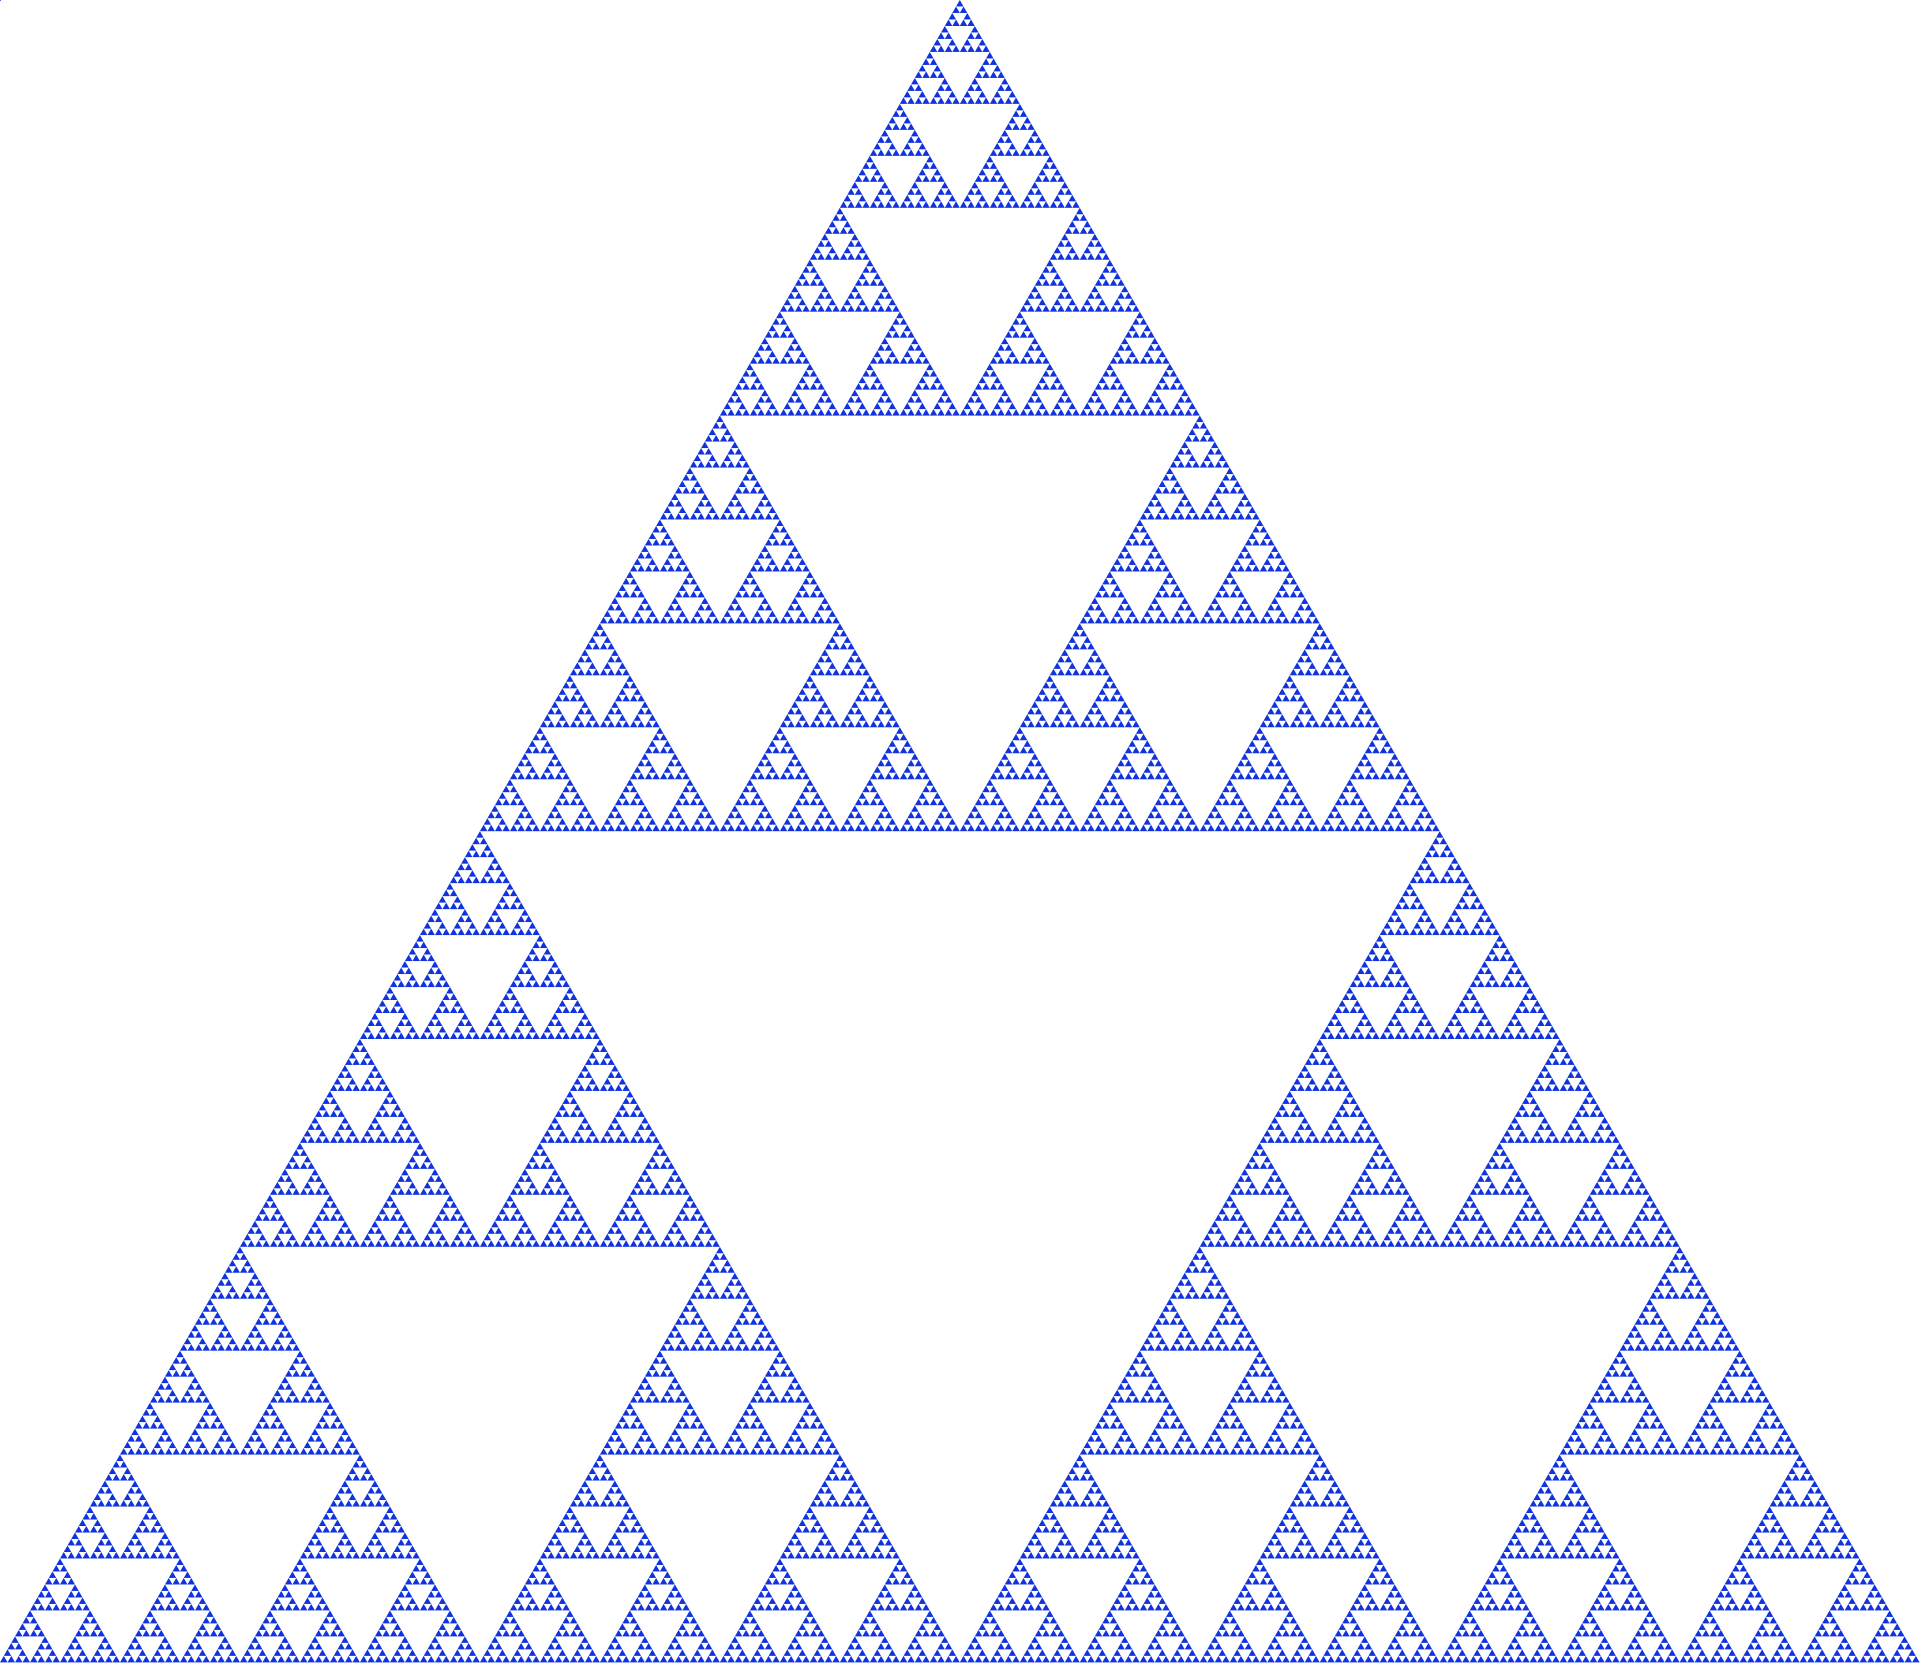
\includegraphics[width=0.5\textwidth]{images/Sierpinski_triangle.svg.png}
    \caption{Serpi\'{n}ski triangle. \cite{img:sierpinski}}
    \label{fig:sierpinski}
\end{figure}
\newpage
\begin{example}{(Koch curve).}
    There are four similarities each with ratio $r=1/3$. By Moran's theorem: $4\cdot(1/3)^s=1$, so $s=\log4/\log3\approx1.26185951$
\end{example}
\begin{figure}[h]
    \centering
    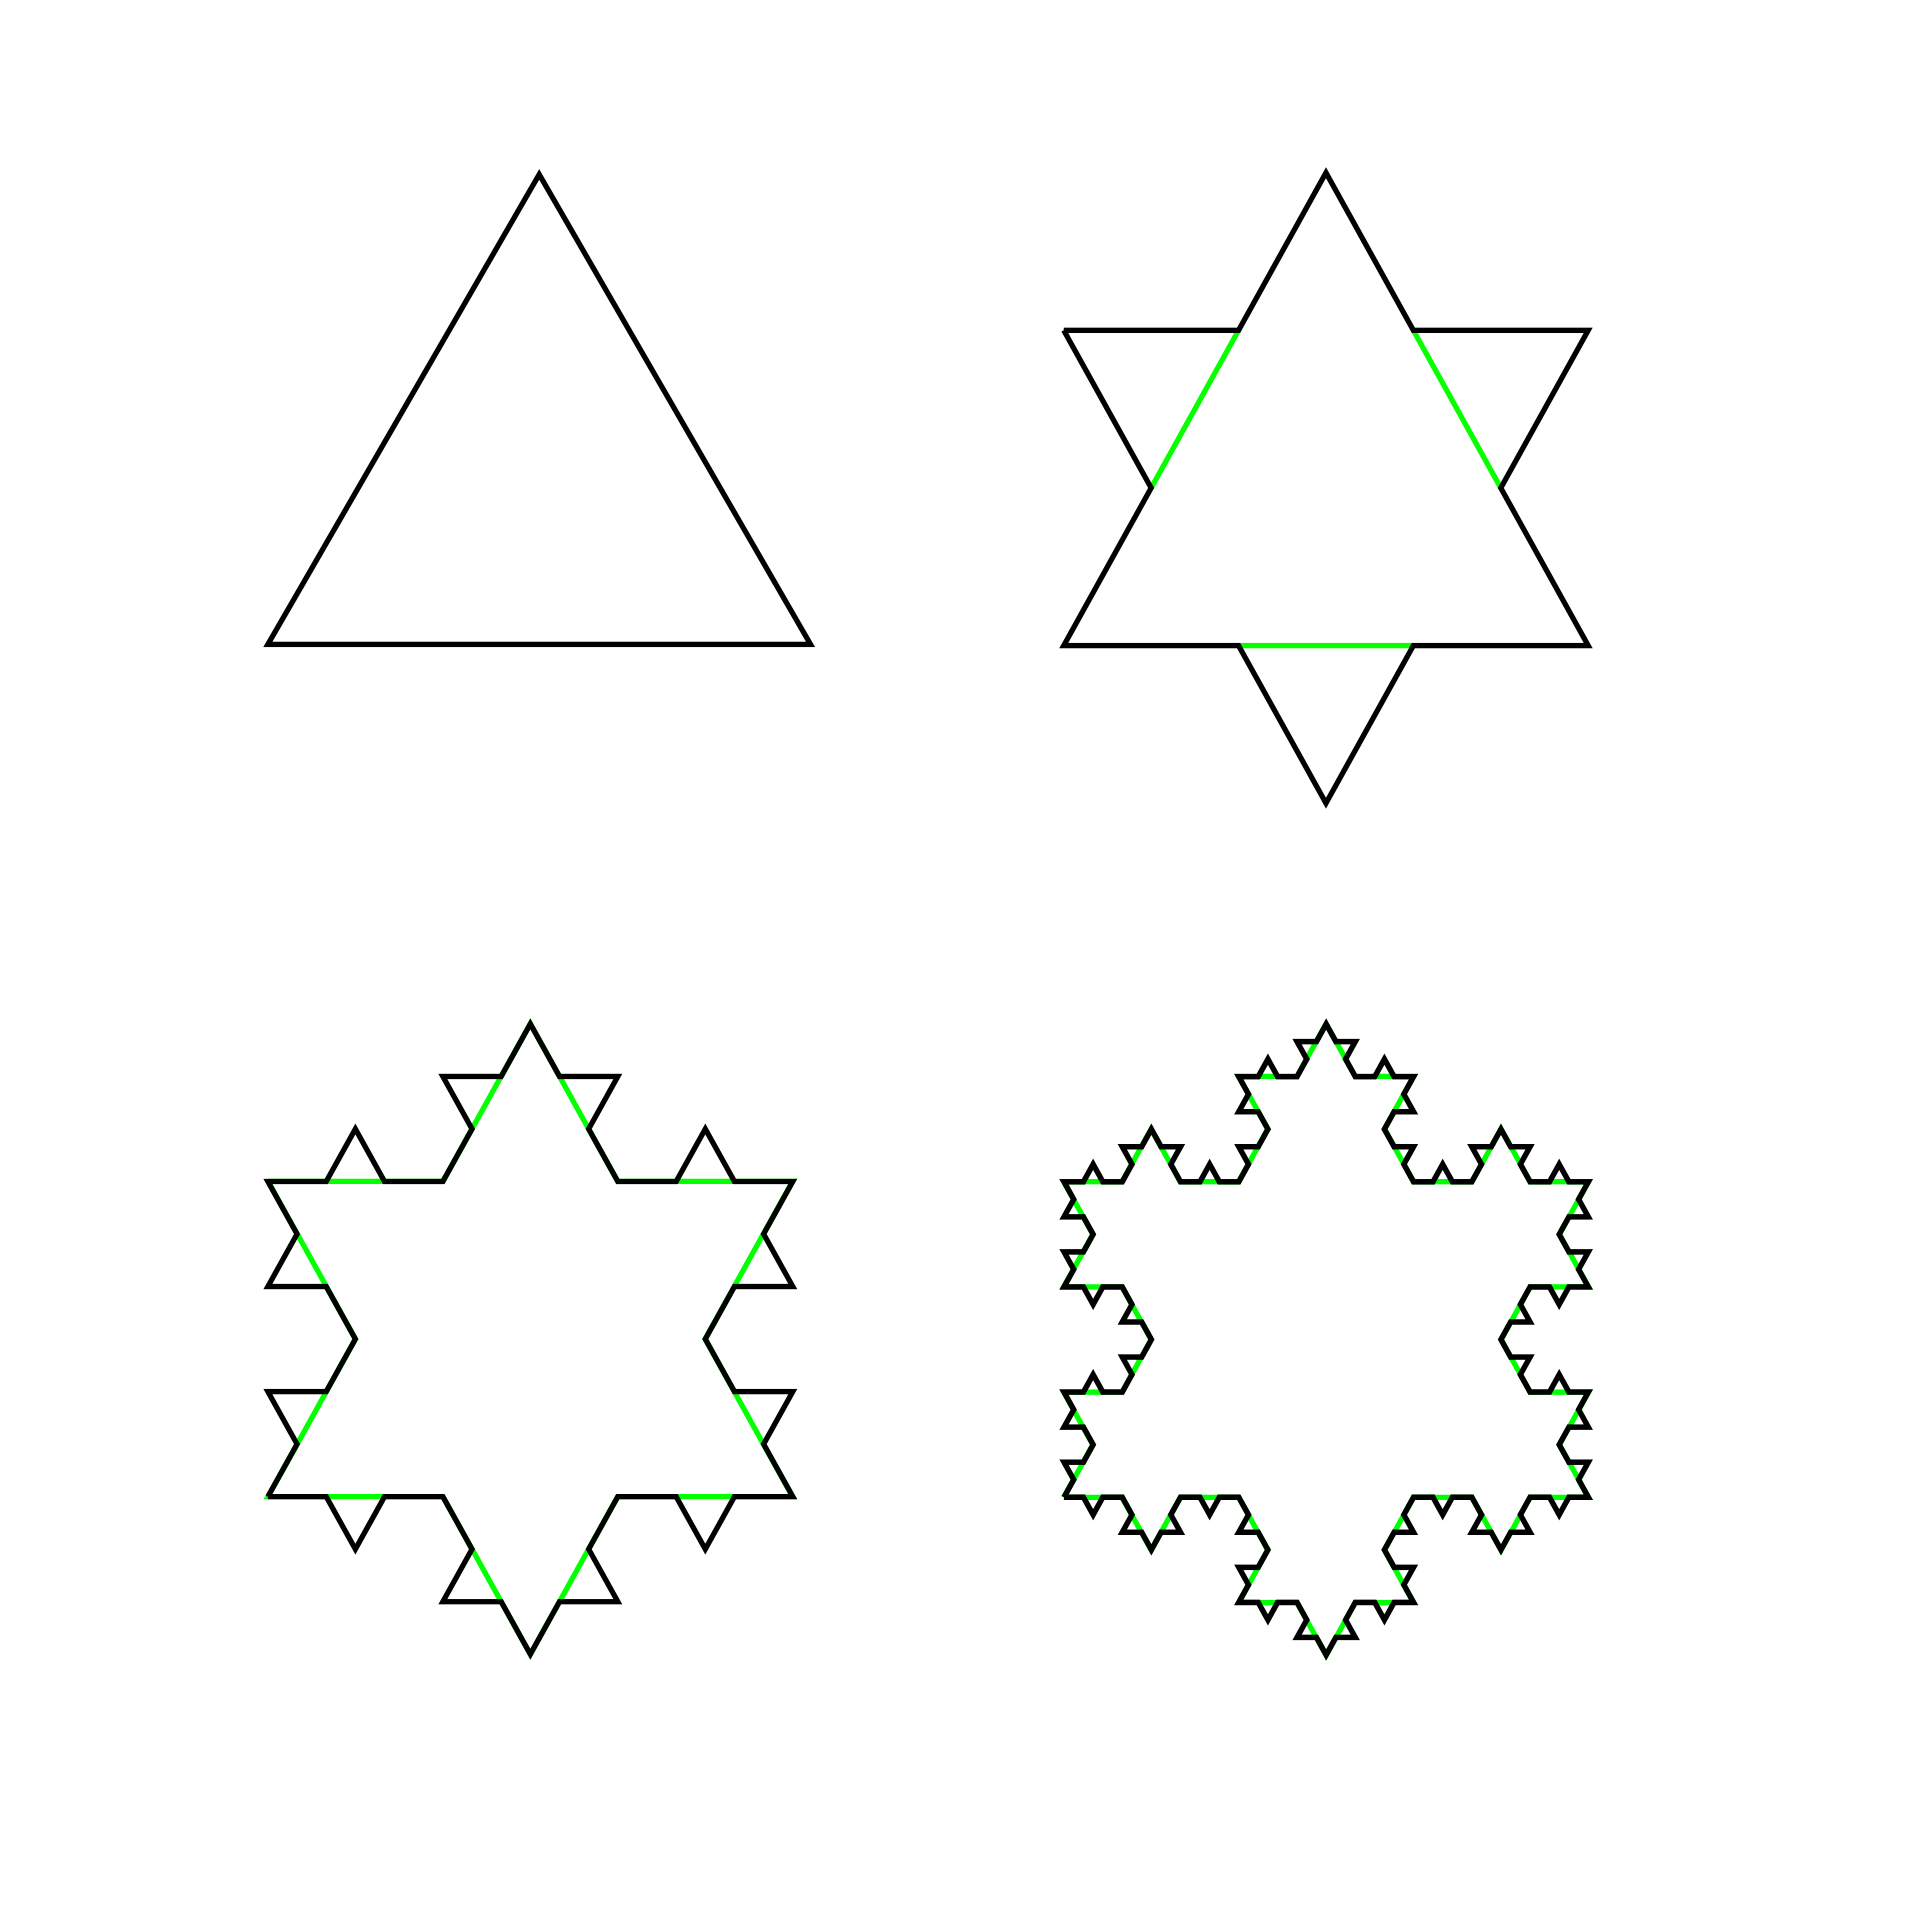
\includegraphics[width=0.5\textwidth]{images/KochFlake.svg.png}
    \caption{Koch snowflake with 4 iterations. \cite{img:koch}}
    \label{fig:koch}
\end{figure}
\newpage
\newpage
\section{L-systems}
Moran's theorem gives the dimension of an IFS attractor, but specifying an IFS by hand is long. 
L-systems\footnote{Introduced by Lindenmayer in 1968 tomodel plant growth; see \cite{prusinkiewicz1990abop}.} provide a purely symbolic description of the same objects, from which $\lambda$ and $k$ can be recovered almost mechanically. 
This gives us a family of fractals with exactly known dimension, which we will use in \S9 to validate the box-counting estimator.

\subsection{Definition}
\begin{definition}{(D0L-system).}
    A \textbf{deterministic context-free L-system} is a triple $G=(V,\omega,P)$ where $V$ is a finite alphabet, $\omega\in V^+$ is the \textbf{axiom}, and $P:V\to V^*$ assigns a \textbf{production} to each symbol. Writing $\omega_0=\omega$, the word $\omega_{n+1}$ is obtained from $\omega_n$ by replacing \emph{every} symbol simultaneously by its production.
\end{definition}
\noindent We need parallel writing here so that every part of the word changes at the same rate for self-similarity.

\subsection{Turtle interpretation}
\begin{definition}{(Turtle interpretation).}
    Fix a step length $\ell>0$ and a turning angle $\delta$. A turtle has state
    $(x,y,\alpha)\in\R^2\times[0,2\pi)$. Reading a word left to right:
    \begin{itemize}
        \item \texttt{F}: move forward $\ell$, drawing a segment;
        \item \texttt{f}: move forward $\ell$ without drawing;
        \item \texttt{+}, \texttt{-}: turn left, right by $\delta$.
    \end{itemize}
    Symbols with no geometric interpretation are ignored. Write $\gamma_n$ for the drawn figure of $\omega_n$ with step length $\ell_n$.
\end{definition}
\noindent Note that the grammar alone does not determine a curve: the angle
$\delta$ and the choice of $\ell_n$ are geometric data supplied separately.

\subsection{The growth matrix}
\begin{definition}{(Substitution matrix).}
    For $G=(V,\omega,P)$ with $V=\{a_1,\dots,a_m\}$, the \textbf{substitution
    matrix} $M\in\N^{m\times m}$ is given by
    \[
    M_{ij}=\#\{\text{occurrences of } a_j \text{ in } P(a_i)\}.
    \]
\end{definition}
\subsection{Growth of the substitution matrix}
Let $v_n\in\N^m$ record the symbol counts of $\omega_n$, so that $v_{n+1}=v_nM$
and hence $v_n=v_0M^n$. Since box-counting sees only the drawn segments, the
quantity of interest is the \texttt{F}-component of $v_n$.

\begin{theorem}{(Perron--Frobenius).}\label{thm:pf}
    Let $M$ be a square matrix with non-negative entries and spectral radius
    $\lambda=\max_i|\lambda_i|$. Then $\lambda$ is an eigenvalue of $M$, with a
    non-negative eigenvector. If moreover $M$ is irreducible, then $\lambda$ is
    simple and its eigenvector may be taken strictly positive. If $M$ is
    \textbf{primitive} --- irreducible with $M^m>0$ for some $m$ --- then
    additionally $\lambda>|\lambda_i|$ for every other eigenvalue.
\end{theorem}

\noindent Expanding $v_0$ in a basis of left eigenvectors gives
$v_n=\sum_i c_i\lambda_i^nu_i$; dividing by $\lambda^n$ shows every subdominant
term vanishes, so $v_n\sim c_1\lambda^nu_1$ and $\|v_n\|=\Theta(\lambda^n)$.
Primitivity is what rules out a complex or sign-alternating eigenvalue of the
same modulus as $\lambda$, which would make $\|v_n\|/\lambda^n$ oscillate
rather than converge. Irreducibility is not sufficient: an irreducible matrix of
period $p$ has eigenvalues $\lambda e^{2\pi ij/p}$, all of modulus $\lambda$.
An extreme case would be $M=\left(\begin{smallmatrix}0&1\\1&0\end{smallmatrix}\right)$,
where the symbol counts simply swap at every step.

\begin{example}{(Hilbert).}\label{ex:hilbert}
    The Hilbert curve is generated by
    \[
    A\to\texttt{+BF-AFA-FB+},\qquad B\to\texttt{-AF+BFB+FA-},\qquad
    \delta=90^\circ,
    \]
    with $\texttt{F}\to\texttt{F}$. Here $A$ and $B$ carry the recursion and are
    ignored by the turtle; two are needed because the sub-curves come in mirror-image pairs. On $(A,B,F)$,
    \[
    M=\begin{pmatrix}2&2&3\\2&2&3\\0&0&1\end{pmatrix}.
    \]
    With $v_0=(1,0,0)$ the counts are $v_1=(2,2,3)$, $v_2=(8,8,15)$,
    $v_3=(32,32,63)$, so the number of drawn segments at level $n$ is $4^n-1$.
    The eigenvalues of $M$ are $4,1,0$, and correspondingly
    $F_n=1\cdot4^n-1\cdot1^n$: the dominant eigenvalue sets the growth rate and
    the subdominant one contributes the correction. Note $v_3\approx
    32\cdot(1,1,2)$, the dominant left eigenvector.
\end{example}

\begin{remark}{(Reducibility).}\label{rem:reducible}
    The matrix above is reducible: the associated digraph has edges
    $A,B\to F$ but none from $F$ back, so it is not strongly connected and the
    strong form of \ref{thm:pf} does not apply. The conclusion survives because
    \texttt{F} is reachable from the block $\{A,B\}$ carrying the dominant
    eigenvalue. In general it suffices that the drawn symbols be reachable from
    the dominant block.
\end{remark}

\begin{proposition}{(Dimension of a D0L-system).}\label{prop:d0l}
    Let $G$ be a D0L-system with substitution matrix $M$, write
    $F_n=\#\{\text{drawn symbols in }\omega_n\}$, and let
    \[
      \lambda=\lim_{n\to\infty}F_n^{1/n}
    \]
    be the growth rate of the drawn symbols, assumed to exist. Suppose the
    turtle interpretation
    admits a scaling factor $k>1$, meaning that $\gamma_n$ is drawn with step
    length $\ell_n=k^{-n}$. Then
    \[
    \Bd(K)\leq\frac{\log\lambda}{\log k},
    \]
    where $K=\lim_n\gamma_n$, with equality when the induced IFS satisfies the OSC.
\end{proposition}
\begin{proof}
    The level-$n$ figure is a union of $F_n$ segments of length $k^{-n}$, and $F_n=\lambda^{n+o(n)}$ by the definition of $\lambda$.
    Covering $K$ at scale $\eps=k^{-n}$ requires $N(\eps)=\lambda^{n+o(n)}$ boxes, so
    \[
    \frac{\log N(\eps)}{\log(1/\eps)}
      =\frac{n\log\lambda+o(n)}{n\log k}
      \longrightarrow\frac{\log\lambda}{\log k}.
    \]
    Under the OSC the drawn segments overlap only at endpoints, so the count is
    $\lambda^{n-o(n)}$ from below as well and the limit is attained.
\end{proof}

\noindent Two caveats. First, $\lim F_n^{1/n}$ need not exist: with
$M=\left(\begin{smallmatrix}0&1\\1&0\end{smallmatrix}\right)$ and one symbol
drawn, $F_n$ runs $1,0,1,0,\dots$ It does exist when the part of $M$ producing
the drawn symbols is primitive.

Second, $\lambda$ is the growth rate of the \emph{drawn} symbols, which need not
be $\rho(M)$, the growth rate of all symbols. Only symbols that are reachable
from the axiom and eventually produce a drawn symbol count, so
\[
  \lambda=\max_{C\in\mathcal{S}}\rho(C),
\]
where $\mathcal{S}$ is the set of strongly connected components of $M$ with
both properties. This equals $\rho(M)$ for every system in
Table~\ref{tab:lsystems} except Cantor (Remark~\ref{rem:undrawn}).

So Proposition~\ref{prop:d0l} splits the dimension into two independent parts:
$\lambda$ comes from the grammar alone, and $k$ from the geometry ($\delta$ and how far one production carries the turtle).

\begin{remark}[Why the growth rate, not a symbol count]
    For Koch ($\texttt{F}\to\texttt{F+F-{}-F+F}$), $\lambda=4$ is just the
    number of \texttt{F}s in the production. For Hilbert
    (Example~\ref{ex:hilbert}) this doesn't work: each production has 3
    \texttt{F}s, suggesting $\log3/\log2\approx1.585$, but the $A$s and $B$s
    also turn into \texttt{F}s at the next level, so the true growth rate is
    $4$ and the dimension $\log4/\log2=2$.
\end{remark}

\subsection{A validation family}
\begin{table}[h]
\centering
\begin{tabular}{llccl}
\hline
Fractal & Production(s) & $\delta$ & $\lambda/k$ & Dimension \\
\hline
Cantor & \texttt{F}$\to$\texttt{FfF}, \texttt{f}$\to$\texttt{fff}
    & --- & $2/3$ & $0.630930$ \\
Koch & \texttt{F}$\to$\texttt{F+F-{}-F+F}
    & $60^\circ$ & $4/3$ & $1.261860$ \\
Minkowski & \texttt{F}$\to$\texttt{F+F-F-FF+F+F-F}
    & $90^\circ$ & $8/4$ & $1.5$ \\
Arrowhead & \texttt{A}$\to$\texttt{B-A-B}, \texttt{B}$\to$\texttt{A+B+A}
    & $60^\circ$ & $3/2$ & $1.584963$ \\
Peano & \texttt{F}$\to$\texttt{F+F-F-F-F+F+F+F-F}
    & $90^\circ$ & $9/3$ & $2$ \\
Hilbert & see \ref{ex:hilbert}
    & $90^\circ$ & $4/2$ & $2$ \\
\hline
\end{tabular}
\caption{L-systems with exactly known dimension, used in \S9.}
\label{tab:lsystems}
\end{table}

\noindent Their dimensions span $[0.63,\,2]$ and are known exactly, so they make a good test set for the estimator.
\newpage
\section{Hilbert curve}
This is possibly my favourite fractal that I'd like to explore. It is essentially a mapping from 1D to 2D space (earning the title space-filling curve).
\subsection{Construction}
The Hilbert curve is a continuous surjection $\gamma:[0,1]\rightarrow[0,1]^2$ constructed as the uniform limit of a sequence of piecewise-linear approximations $\gamma_n$. At order $n$, the curve $\gamma_n$ traverses all $4^n$ cells of a $2^n\times2^n$ grid, connecting cell centres via a path that divides each grid cell into four sub-cells connected in a U-shape, rotated and reflected to ensure the overall path shape is continuous. From this we can see directly that it has dimension 2 (even though its not closed), since we have 4 similarities with ratio $1/2$, giving $\log4/\log2 = 2$.

\begin{figure}[h]
    \centering
    \begin{subfigure}[b]{0.3\textwidth}
        \centering
        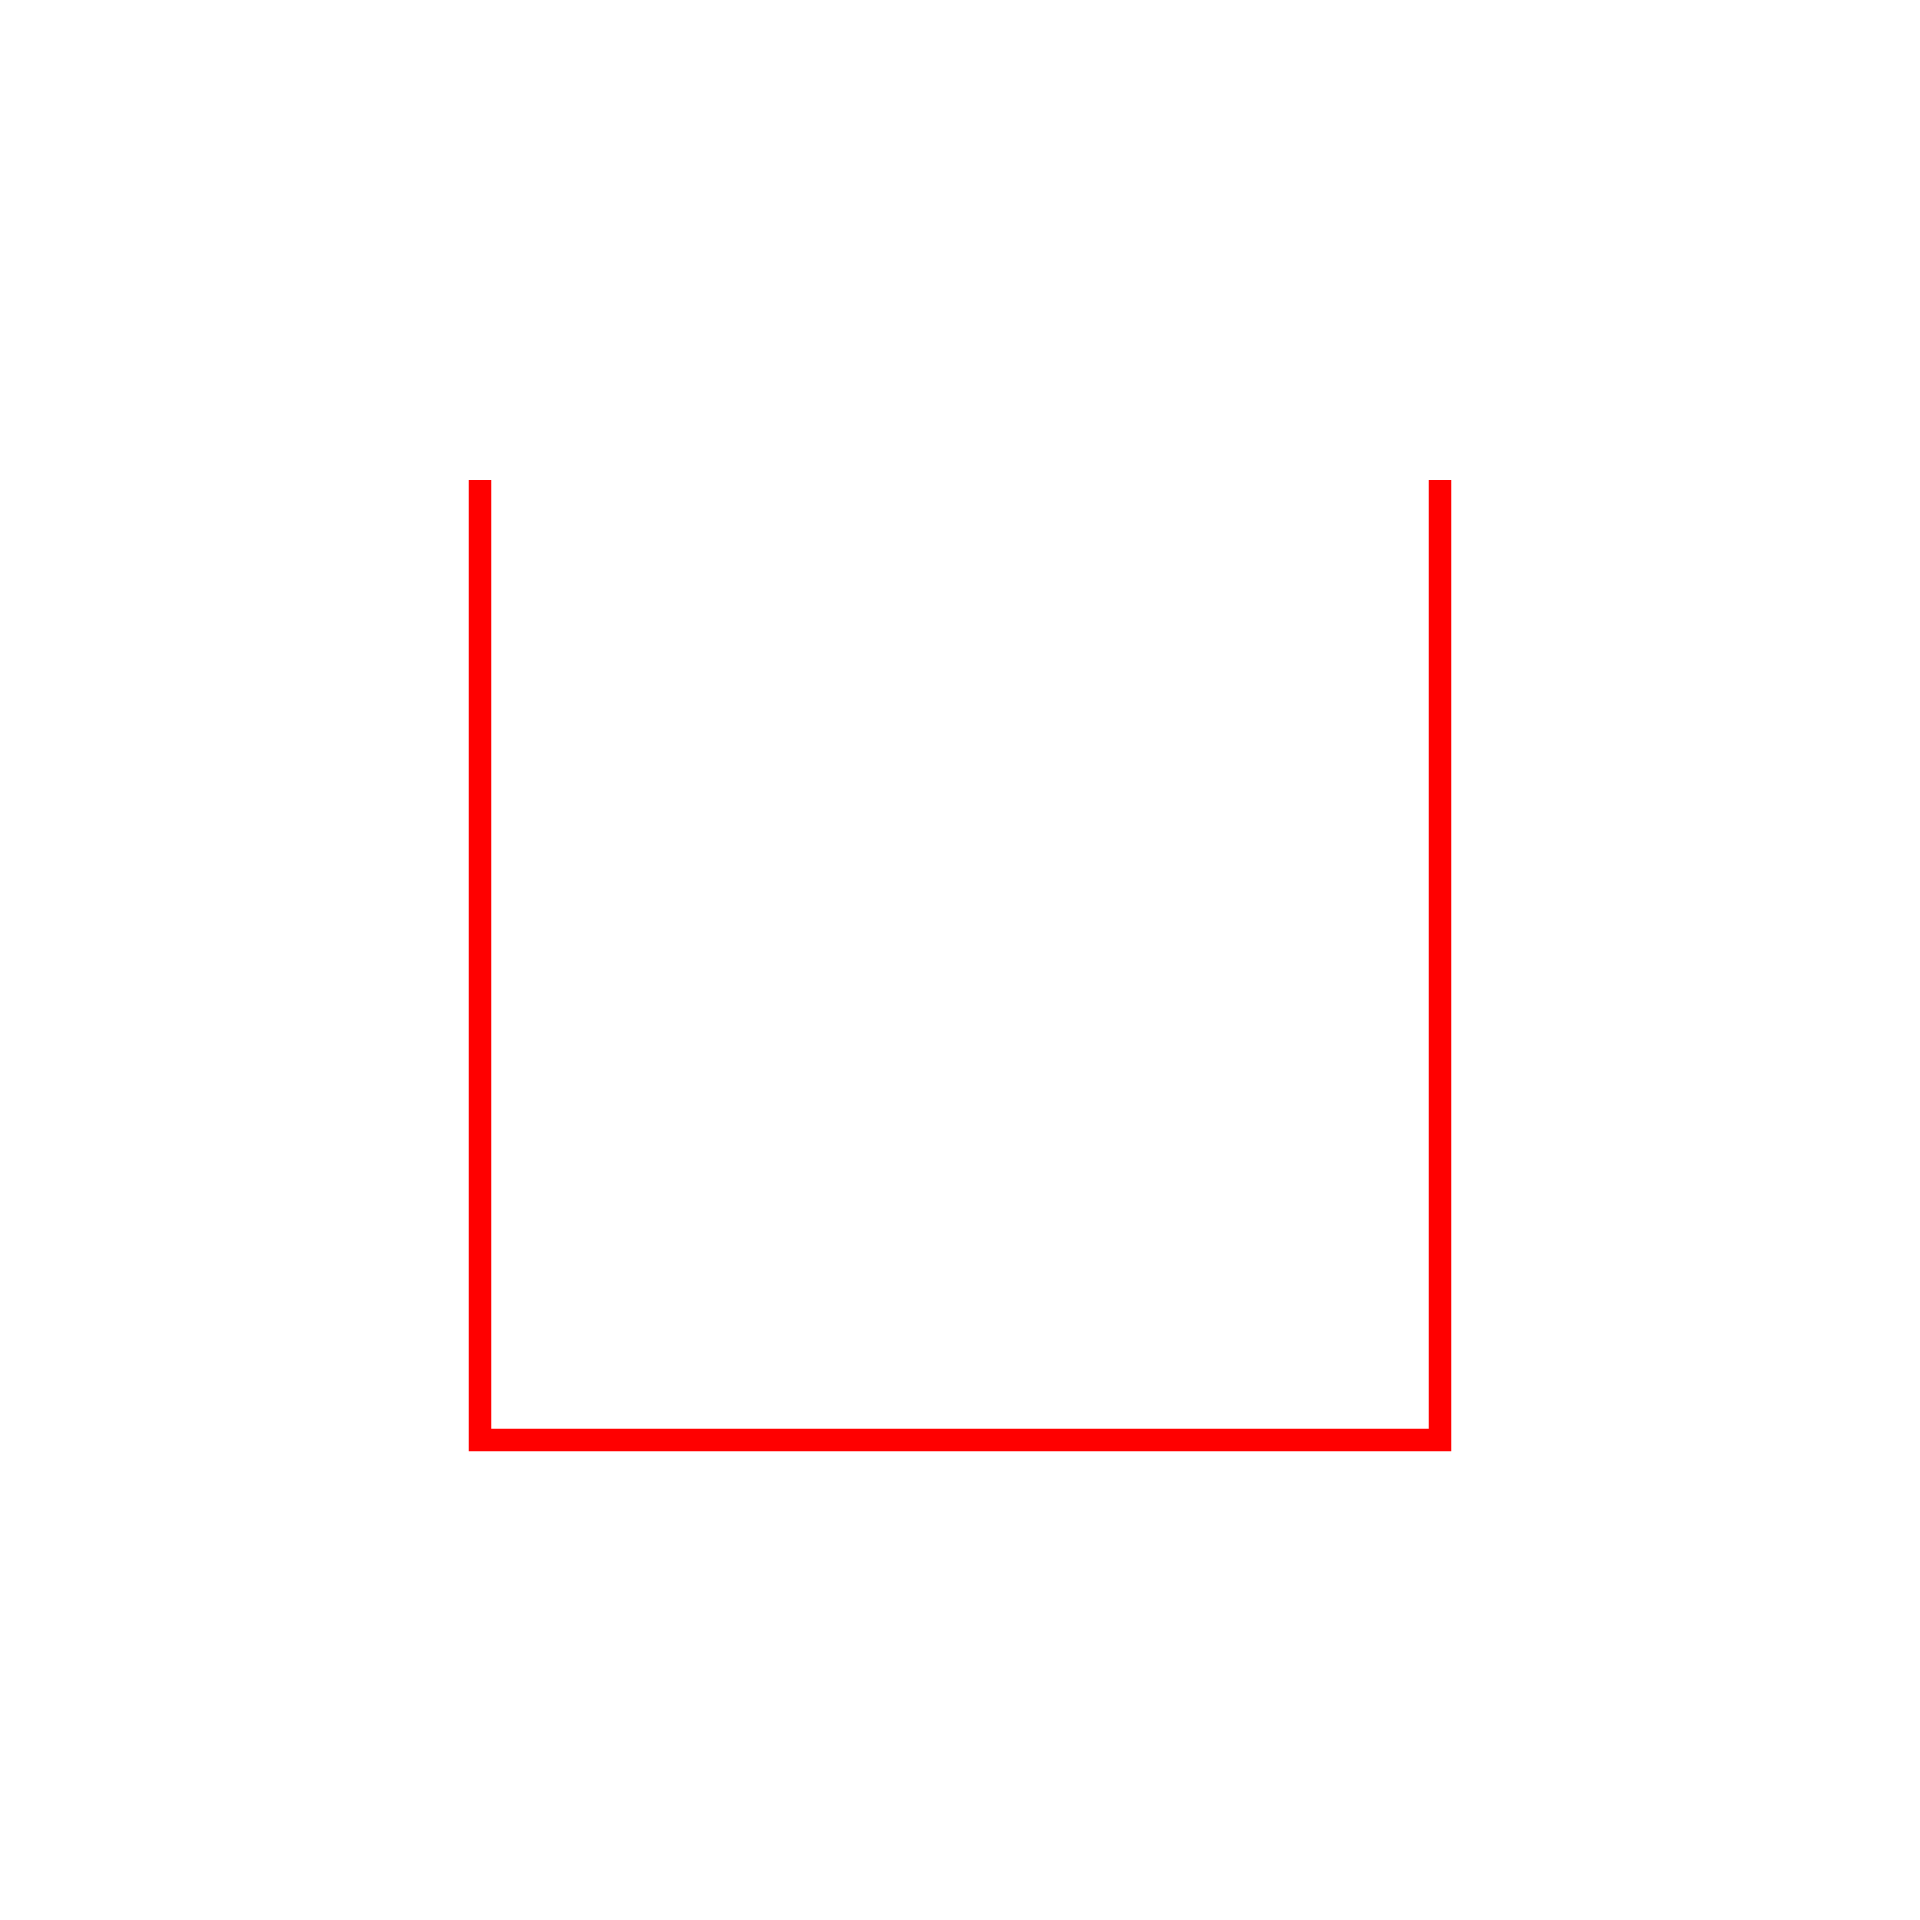
\includegraphics[width=\textwidth]{images/Hilbert_curve_1.svg.png}
        \caption{First iteration.}
        \label{fig:h1}
    \end{subfigure}
    \hfill
    \begin{subfigure}[b]{0.3\textwidth}
        \centering
        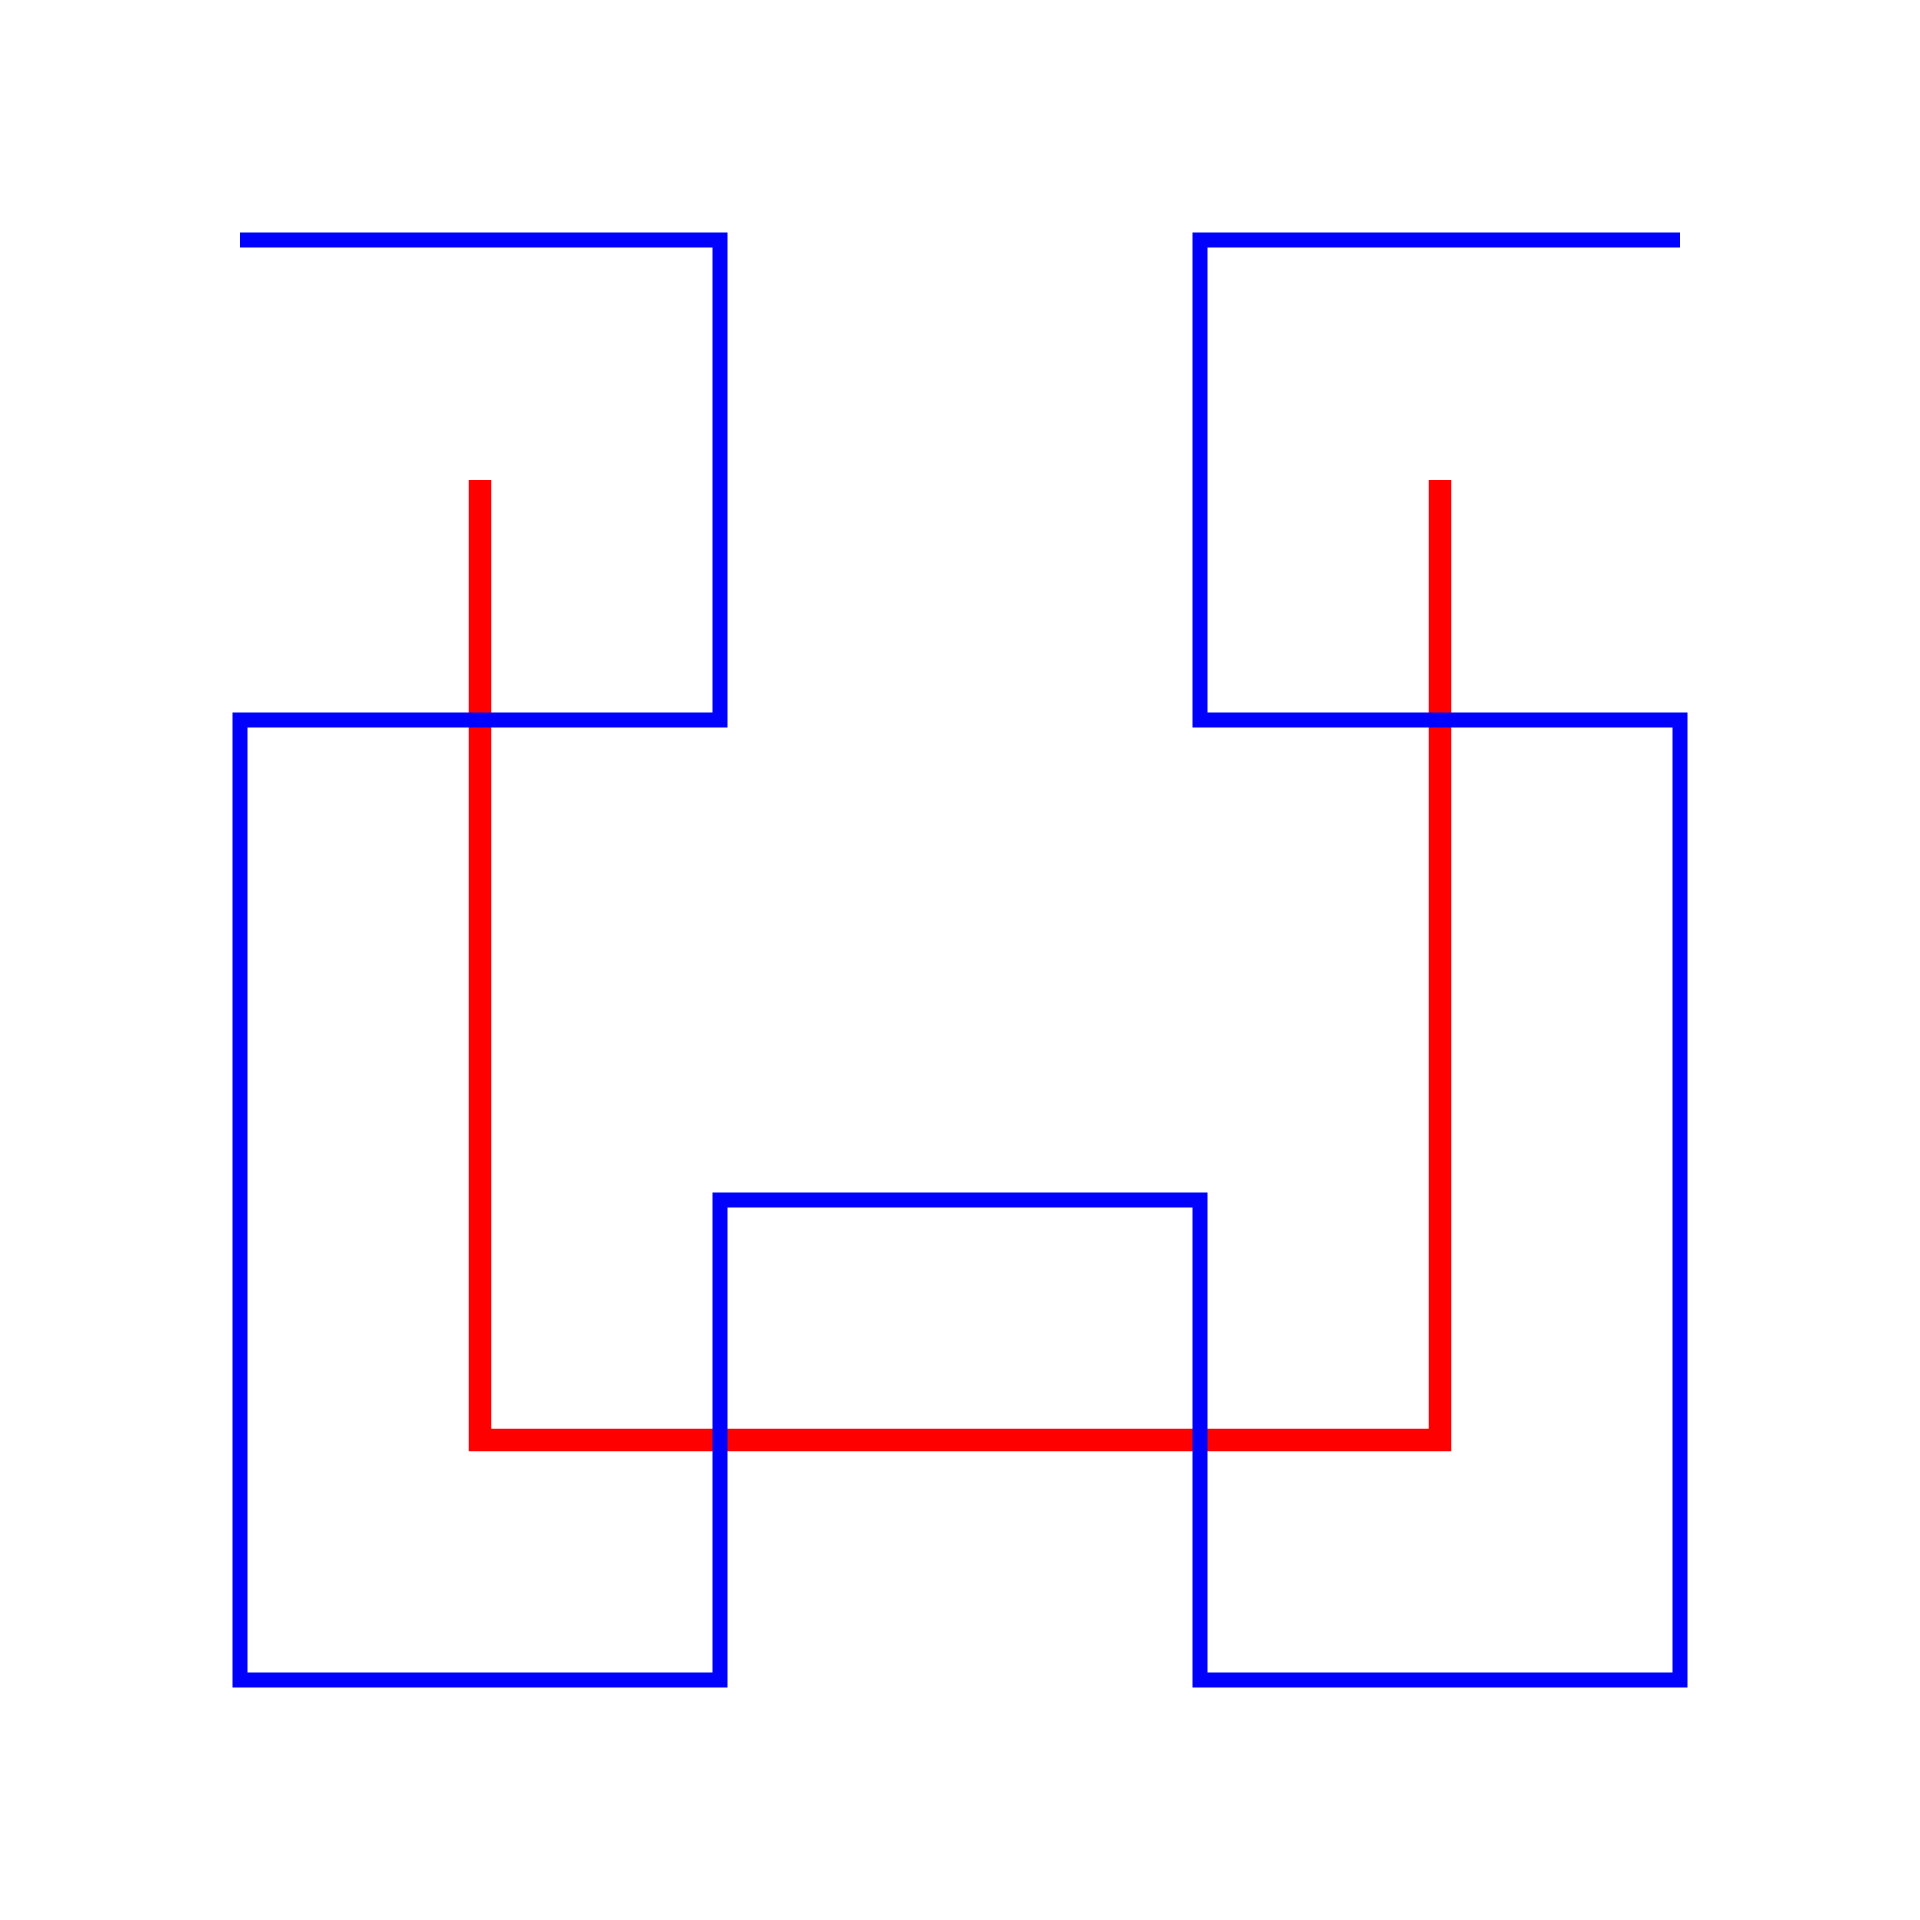
\includegraphics[width=\textwidth]{images/Hilbert_curve_2.svg.png}
        \caption{Iterations 1 and 2.}
        \label{fig:h2}
    \end{subfigure}
    \hfill
    \begin{subfigure}[b]{0.3\textwidth}
        \centering
        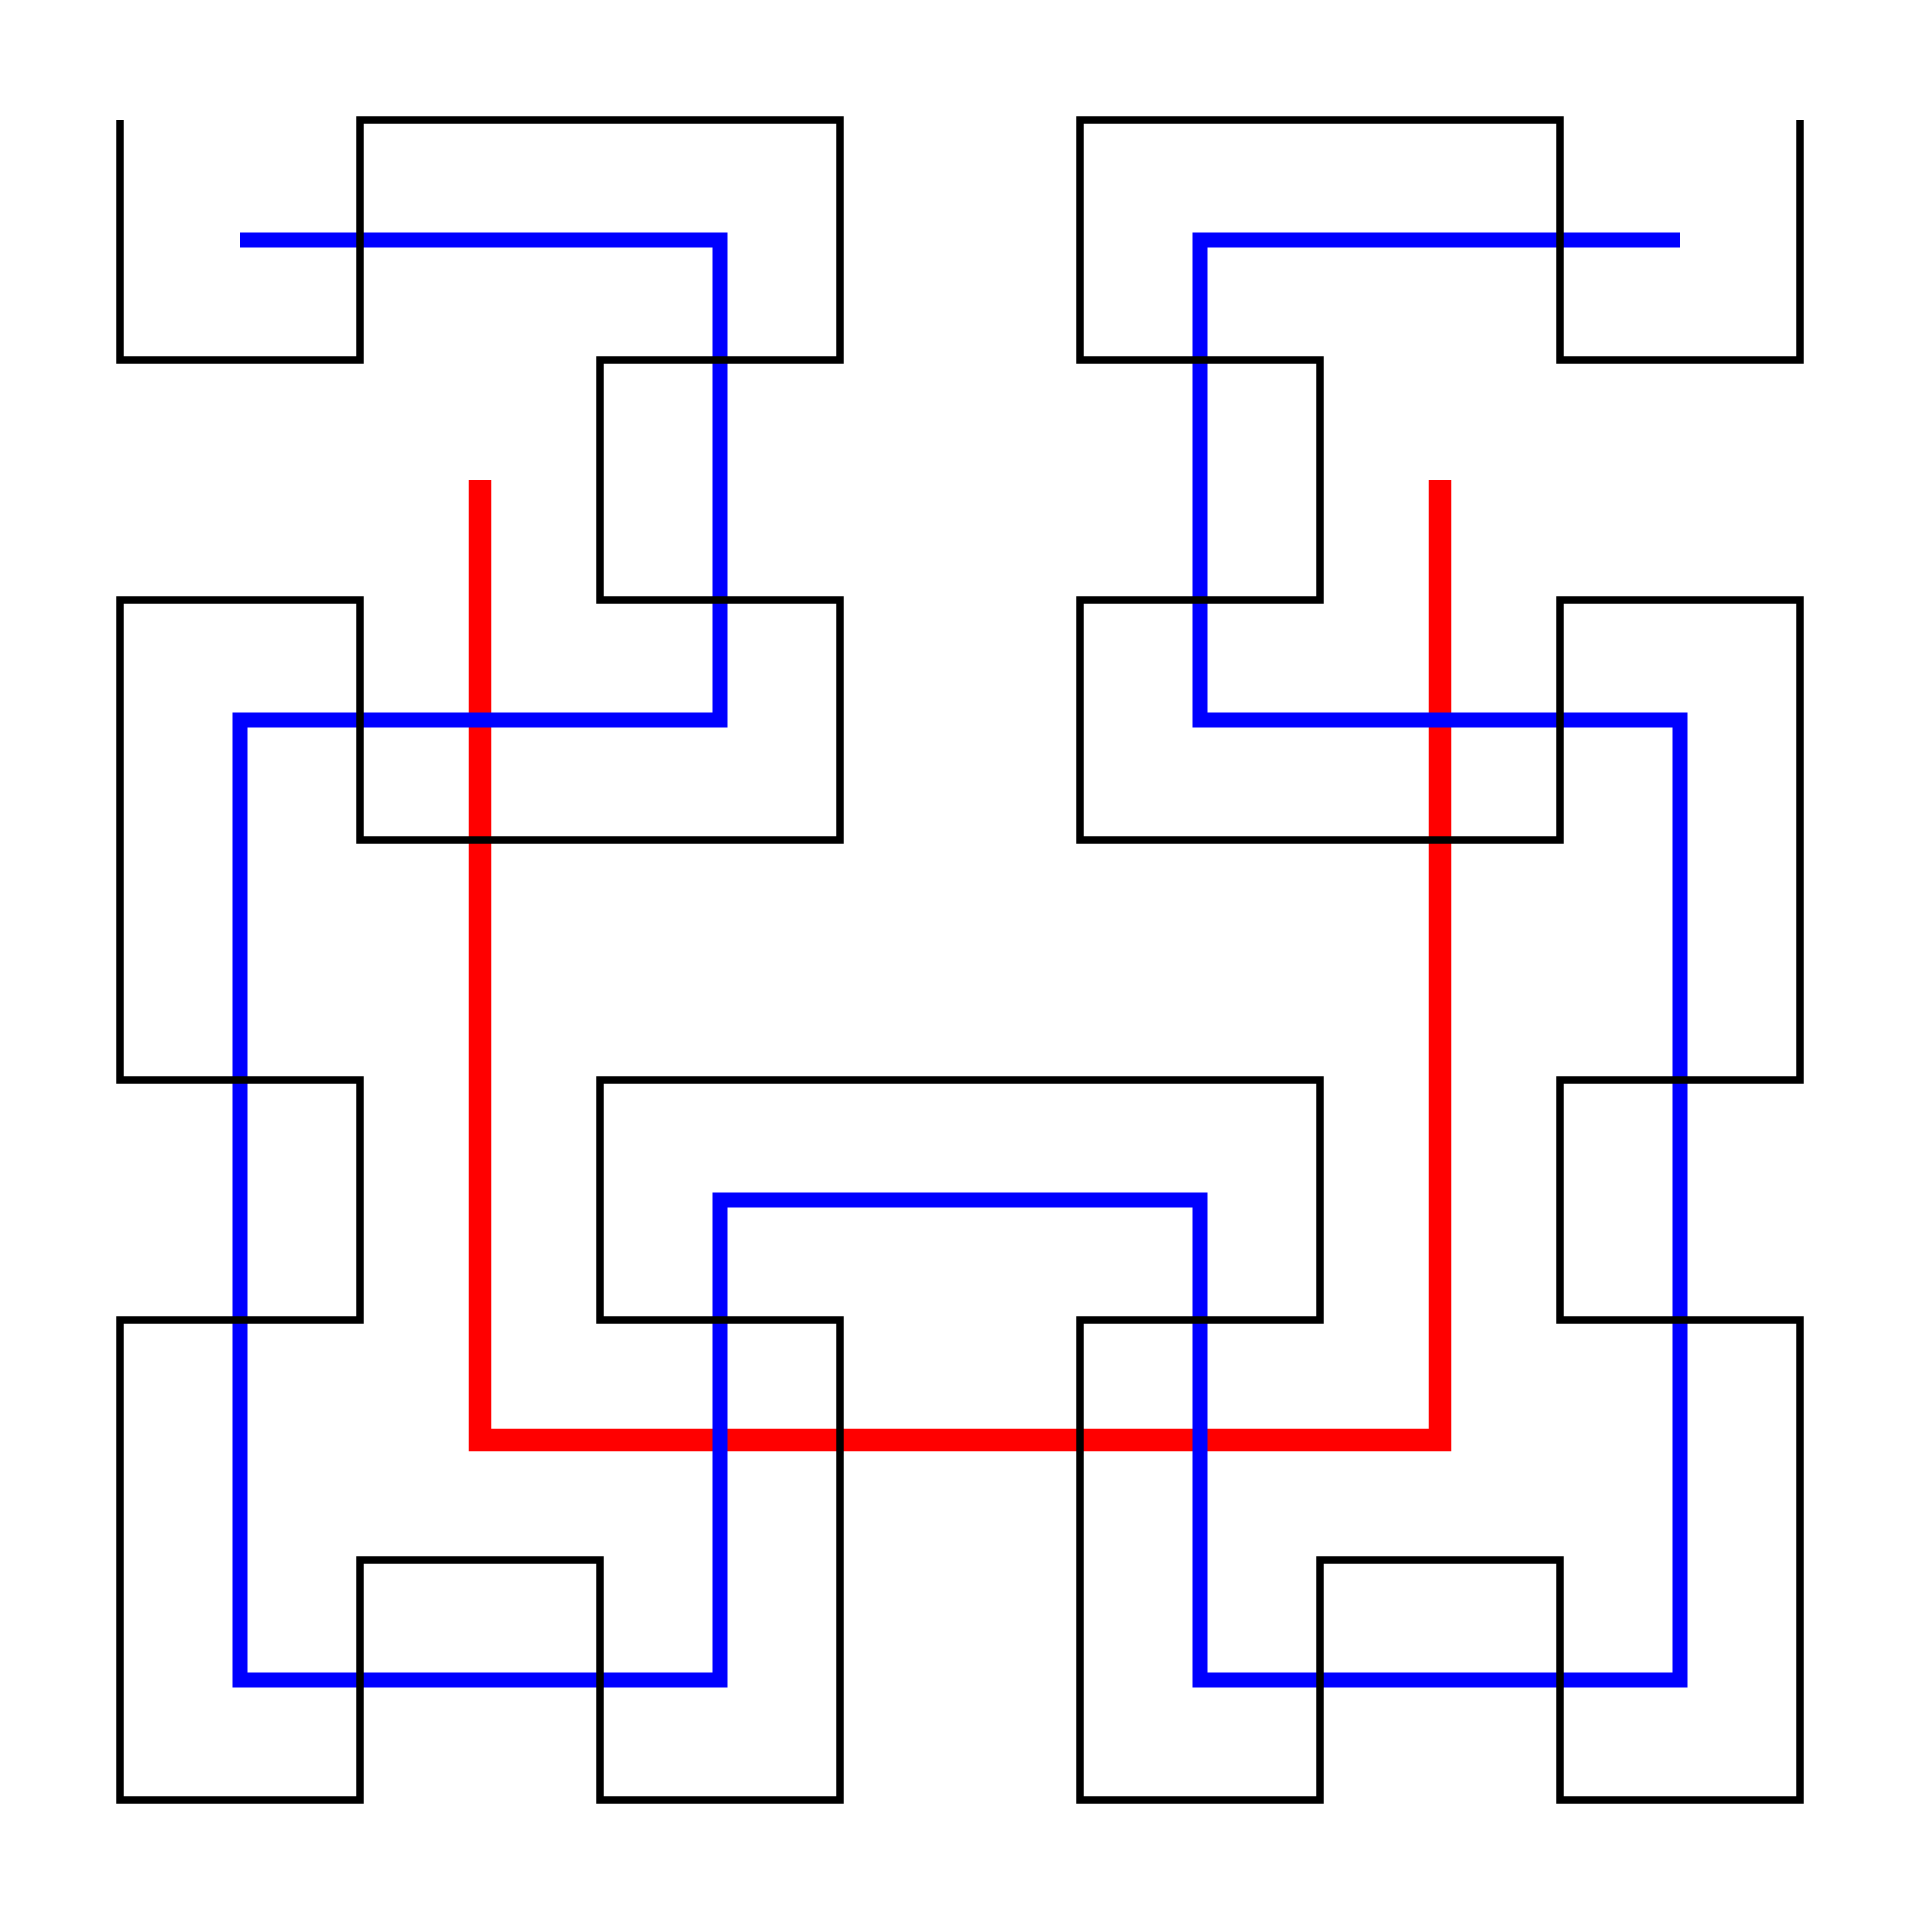
\includegraphics[width=\textwidth]{images/Hilbert_curve_3.svg.png}
        \caption{Iterations 1 to 3.}
        \label{fig:h3}
    \end{subfigure}
    \caption{Hilbert curve approximations. \cite{img:example}}
\end{figure}

\subsection{Properties of the limit curve}

\newpage
\section{Computational Estimation}
\label{sec:computational}

Everything so far has computed dimensions \emph{from} a description: Moran's
equation from an IFS, $\log\lambda/\log k$ from a grammar. However, you can also to calculate it from just a picture.

\begin{description}
    \item[Mode A - from the grammar.] Recover $\lambda$ and $k$ from the
    productions and the turtle, then apply \ref{prop:d0l}. Exact and fast but requires the rule.
    \item[Mode B - from the picture.] Box-count the drawn segments and fit
    the scaling window. Approximate and expensive, but done without grammar, so it is the only method for a
    picture (e.g. a coastline, a micrograph, a point cloud).
\end{description}

\noindent They share no input beyond the system itself and no code beyond the
tracer, so their agreement is independent evidence that they are both right. However, they are nowhere near the same accuracy:
Mode A reproduces every known dimension in the library exactly (Table \ref{tab:growth}); 
Mode B is exact only on Hilbert, within $0.005$ on one more, within $0.034$ on six others, and very wrong twice. (see table \S\ref{sec:estimates})

% ─────────────────────────────────────────────────────────────────────────────
\subsection{Mode A: recovering \texorpdfstring{$\lambda$}{lambda} and
\texorpdfstring{$k$}{k} from the grammar}
\label{sec:modea}

The computation is the following eight steps.

\begin{enumerate}
    \item \textbf{Symbol table.} Fix which symbols draw, which move without drawing, which only turn, and which push or pop the stack. 
    This is kept separate from the grammar because the same letter can draw in one system and not in another: Hilbert's A and B draw nothing, while the Arrowhead's do.

    \item \textbf{Matrix alphabet.} Drop the orientation symbols
    $\texttt{+},\texttt{-},\texttt{|},\texttt{[},\texttt{]}$: they have no
    production and contribute no length, so keeping them would pad $M$ with
    dead rows. This is what makes Hilbert's matrix $3\times3$ over
    $\{A,B,F\}$ in \ref{ex:hilbert} rather than $5\times5$.

    \item \textbf{Substitution matrix.} $M_{ij}=\#\{a_j\text{ in }P(a_i)\}$,
    one pass over the productions.

    \item \textbf{$\lambda$, the growth rate of the drawn symbols} - factor by which number of drawn segments multiplies between levels. Iterate
    $v_{n+1}=v_nM$ in exact integer arithmetic and take the ratio of the drawn
    components at two successive levels, deep enough that the subdominant terms
    have decayed (ratio stops changing). \ref{prop:d0l} defines $\lambda$ as $\lim F_n^{1/n}$; the
    ratio $F_{n+1}/F_n$ is used instead because it converges much faster, and
    the two agree whenever the component generating the symbols is primitive, (it is for all systems in the library).
    The counts are kept as integers, so $\lambda$ comes out exact whenever it is rational.
    Floating point would give the same answer to full precision, so this is tidiness rather than necessity. Note that $\lambda$ is not in general $\rho(M)$ --- see Remark \ref{rem:undrawn}.

    \item \textbf{$\rho(M)$, for comparison} --- the spectral radius of the whole
    matrix, i.e.\ the growth rate of all symbols, drawn or not. It usually equals
    $\lambda$, and printing both shows when it does not (Cantor). The code also
    tests whether $M$'s digraph is strongly connected;
    when it is not, as for Hilbert and Cantor, the code prints a warning (Remark~\ref{rem:reducible}).

    \item \textbf{$k$, the scaling factor.} Two routes; \S\ref{sec:k}.

    \item \textbf{Branching test.} If any symbol pushes or pops the turtle state
(\texttt{[}, \texttt{]}), the figure is no longer built from scaled copies
laid end to end, and branches may overlap, so Moran's theorem does not apply.
$\lambda$ and $k$ are still computed, but $\log\lambda/\log k$ is not reported
as a dimension. This is what's going on with the \texttt{plant} row of Table~\ref{tab:growth}.

    \item \textbf{Dimension.} $\log\lambda/\log k$.
\end{enumerate}

\begin{remark}[Growth rate v.s. spectral radius]
\label{rem:undrawn}
    The $\lambda$ of \ref{prop:d0l} is the growth rate of the \emph{drawn}
    symbols, because those are the only ones box counting can see. Usually that
    is $\rho(M)$, and the implementation reports both so the two can be
    compared. Cantor is an exception: over $\{\texttt{F},\texttt{f}\}$ the system
    $\texttt{F}\to\texttt{FfF}$, $\texttt{f}\to\texttt{fff}$ has
    \[
    M=\begin{pmatrix}2&1\\0&3\end{pmatrix},\qquad \rho(M)=3,
    \]
    while the drawn symbols grow as $2^n$. The 3 comes from the
    gaps \texttt{f} multiplying, and since an \texttt{f} never turns into an
    \texttt{F}, that growth never reaches the drawing. Using $\rho(M)$ would
    give $\log3/\log3=1$ instead of $\log2/\log3\approx0.6309$.

    Undrawn symbols should \textbf{\textit{not}} simply ignored, though. Hilbert's \texttt{A} and
    \texttt{B} draw nothing, but they turn into \texttt{F}s at the next level,
    so their growth does reach the drawing, and there $\lambda=\rho(M)=4$
    (Remark~\ref{rem:reducible}). What matters is whether the fast-growing
    symbols eventually produce drawn ones.
\end{remark}

\subsubsection{Two ways to get $k$}
\label{sec:k}

If the production of F moves the turtle k steps from start to end, each level is k times bigger than the last, so k is just the length of that walk:
\[
  k=\bigl|\operatorname{endpoint}(P(\texttt{F}))\bigr|.
\]
For Koch, $P(\texttt{F})=\texttt{F+F-{}-F+F}$ walks out to $(3,0)$, so $k=3$
exactly. If several drawn symbols have productions, they all have to give the same $k$.

This route is unavailable in the case where the recursion is carried by
symbols that draw nothing. Hilbert's $\texttt{F}$ rewrites to itself; all the
structure is in $A$ and $B$, which the turtle ignores. Likewise in the case of the dragon.
There is then no word to walk, and so $k$ has to be read off the drawn figure
instead: trace three successive levels, measure each, and take a ratio of sizes.

So how do we measure the ``size''?
% ─────────────────────────────────────────────────────────────────────────────
\subsection{Measuring the size of a figure: the convex hull}
\label{sec:hull}

The intuitive answer is to use the bounding box: take $\max x-\min x$ and$\max y-\min y$ and call the diagonal the size. 
It is two passes over the points and it is wrong, because the bounding box is not rotation invariant and some of these figures rotate as they grow. 
The Heighway dragon turns $45^\circ$ per level, so its box alternately stands square to the axes and sits at an angle, and the measured ratio alternates with it.

\begin{table}[H]
\centering
\begin{tabular}{rrrr}
\hline
$n$ & box diagonal & diameter & difference \\
 & ratio & ratio & ratio \\
\hline
 6 & $1.4142$ & $1.4518$ & --- \\
 7 & $1.4733$ & $1.4524$ & $1.4538$ \\
 8 & $1.4295$ & $1.4324$ & $1.3883$ \\
 9 & $1.4735$ & $1.4326$ & $1.4329$ \\
10 & $1.3916$ & $1.4232$ & $1.4015$ \\
11 & $1.4509$ & $1.4232$ & $1.4233$ \\
12 & $1.3954$ & $1.4187$ & $1.4079$ \\
13 & $1.4512$ & $1.4187$ & $1.4187$ \\
14 & $1.3866$ & $1.4164$ & $1.4111$ \\
\hline
\end{tabular}
\caption{Successive size ratios for the Heighway dragon, whose true scaling factor is $k=\sqrt2\approx1.414214$. 
The box diagonal keeps jumping above and below $\sqrt2$ and never settles; the diameter gets closer to $\sqrt2$ from above.
The third column differences the diameter, which Remark \ref{rem:differencing} shows is the wrong size to difference for this curve; \ref{rem:endpoint} gives the right one.}
\label{tab:dragon}
\end{table}

\noindent The rotation-invariant replacement is the \textbf{diameter} ---
the greatest distance between any two points of the figure,
$\diam(S)=\sup_{x,y\in S}|x-y|$, which is the same quantity $|U|$ that
Definition 3.1 covers sets with. We can efficiently compute the furthest distance between two points using a convex hull (leetcode mentioned XD).

\begin{lemma}[The diameter is attained at hull vertices]
\label{lem:hull}
    Let $S\subset\R^n$ be bounded with convex hull $H=\operatorname{conv}(S)$.
    Then $\diam(S)=\diam(H)$, and when $S$ is finite the supremum is attained
    at a pair of vertices of $H$.
\end{lemma}
\begin{proof}
    $S\subseteq H$ gives $\diam(S)\leq\diam(H)$. For the converse, fix
    $q\in\overline{H}$. The map $x\mapsto|x-q|$ is convex, so its maximum over
    the compact convex set $\overline{H}$ is attained at an extreme point.
    Applying this in each argument in turn moves both endpoints of any
    diameter-realising pair to extreme points without decreasing the distance.
    For finite $S$ the extreme points of $H$ are vertices, and they lie in $S$,
    so $\diam(H)\leq\diam(S)$.
\end{proof}

\noindent Intuitively: a point inside the hull is an average of hull vertices, and distance to any fixed point can’t exceed the larger of the distances at the points being averaged, so some vertex is always at least as far.

So the search runs over hull vertices, of which these figures have very few: four for the Hilbert curve, ten for the dragon, ten for the Koch curve, against millions of points. 
To compute the hull itself, use Andrew's monotone chain --- 
sort the points lexicographically, sweep once for the lower chain and once for the upper, popping any vertex that doesn't turn counter-clockwise. 
This is just $O(m\log m)$, dominated by the sort (greedy). Collinear points are popped too (think about triangles again), 
so what we get is the corners rather than every boundary point, which keeps the final pairwise search small.

We can now reduce the complexity by a ~ constant factor by just reducing the search space.
Just filter: \emph{for a given $x$, any point strictly between the lowest and the highest point with that $x$ lies on the segment joining them, so it cannot be a vertex.}
Keeping only the per-column extremes costs one lexsort and collapses a lattice curve almost completely.

\begin{table}[H]
\centering
\begin{tabular}{llrrr}
\hline
figure & level & points & candidates & hull vertices \\
\hline
Hilbert & 10 & $2\,097\,150$ & $2\,048$ & $4$ \\
Koch    &  9 & $524\,288$    & $65\,608$ & $10$ \\
Dragon  & 12 & $8\,192$      & $192$     & $10$ \\
\hline
\end{tabular}
\caption{The per-column prefilter. Hilbert and the dragon live on a square lattice, so only two points survive per column. 
Koch's $60^\circ$ turns put its points at many distinct $x$ values, so it keeps a bigger proportion.}
\label{tab:hull}
\end{table}

\noindent The remaining pairwise search over hull vertices is done in blocks of 512, so even a figure with a large hull never uses its full distance matrix in memory (this is just a fallback since all hulls have very few points in the set).
Note that there is actually a better appraoch in $O(h)$ instead of $O(h^2)$ here by rotating calipers but I deemed this an unnecessary improvement for the current scope of the project (especially if you consider \ref{rem:endpoint}).

\begin{remark}[Differencing]
\label{rem:differencing}
    Measuring $k$ as $\diam(\gamma_{n+1})/\diam(\gamma_n)$ converges, but
    slowly, because the diameter is not exactly $Ck^n$. The Hilbert figure at
    level $n$ spans $2^n-1$ steps, so the ratio is
    \[
      \frac{2^{n+1}-1}{2^n-1}=2+\frac{1}{2^n-1},
    \]
    which approaches $2$ from above --- $2.0323$, $2.0159$, $2.0079$,
    $2.0039,\dots$ --- and needs a deep level before it approximates to 4 d.p.. 
    Differencing cancels the constant: if $d_n=Ck^n+A+o(1)$ then
    \[
      \frac{d_{n+1}-d_n}{d_n-d_{n-1}}
      =\frac{Ck^n(k-1)+o(1)}{Ck^{n-1}(k-1)+o(1)}\longrightarrow k,
    \]
    so for Hilbert the ratio is exactly $2$ from $n=2$ onwards.

    Differencing helps only when the correction actually is just a constant.
    For example the dragon's diameter is a case where it is not: the diameter is realised by different pairs of hull vertices at different levels, so the correction oscillates and differencing \emph{amplifies} it. 
    In the third column of Table \ref{tab:dragon} the differenced ratio is worse than the plain one at
    every even level and ties at the odd ones.
\end{remark}

\begin{remark}[Using the displacement]
\label{rem:endpoint}
    Measure instead the \textbf{net displacement} of the drawn figure, from its
    first point to its last. This works better because
    where the curve's endpoints are carried by the similarity it is a pure
    geometric sequence $Ck^n$ with no correction at all, and where the figure
    is a lattice curve it is $Ck^n+A$ with a constant $A$. Both are
    exactly the cases \ref{rem:differencing} handles, so differencing the
    displacement is exact in every case here:
    \begin{center}
    \begin{tabular}{llll}
    \hline
    figure & levels & displacement & differenced ratio \\
    \hline
    Hilbert  & 8--11  & $2^n-1$          & $2.000000000$ \\
    Dragon   & 12--16 & $(\sqrt2)^{\,n}$ & $1.414213562$ \\
    L\'evy C & 10--14 & $(\sqrt2)^{\,n}$ & $1.414213562$ \\
    \hline
    \end{tabular}
    \end{center}
    all to machine precision, against a differenced \emph{diameter} that is out
    by $7.8\times10^{-4}$ for the dragon at level 18 and wanders between
    $1.331$ and $1.476$ for L\'evy C. So we can see here that displacement always wins pretty much.

    \textit{However,} what if displacement is 0? A closed axiom returns the turtle to
    where it started (e.g. Koch snowflake), so there is nothing to difference (or divide by). 
    The implementation therefore computes both sizes and falls back to the diameter. 
    No system in the library actually needs that fallback for its answer (Koch can be calcualted from the exact route) 
    and so the path is only used by the independent cross-check, where the snowflake's differenced diameter returns $3.000000$. 
    The fallback is there for a closed system where $k$ has to be measured, which this library does not happen to contain.
\end{remark}

\noindent With the displacement as the measured size, Mode A lands on its
reference value in every row of Table \ref{tab:growth}.
% ────────────────────
\subsection{Mode A: the whole catalogue}
\label{sec:modearesults}

With both routes for $k$ available, Mode A runs on every system in the
library without drawing anything except where $k$ has to be measured.


\begin{table}[H]
\centering
\begin{tabular}{lrrrlrr}
\hline
system & $\lambda$ & $\rho(M)$ & $k$ & route & dimension & reference \\
\hline
\multicolumn{7}{l}{\itshape the validation family of Table \ref{tab:lsystems}}\\
Cantor    & $2$ & $3$ & $3$        & exact    & $0.630930$ & $0.630930$ \\
Koch      & $4$ & $4$ & $3$        & exact    & $1.261860$ & $1.261860$ \\
Minkowski & $8$ & $8$ & $4$        & exact    & $1.500000$ & $1.500000$ \\
Arrowhead & $3$ & $3$ & $2$        & exact    & $1.584963$ & $1.584963$ \\
Peano     & $9$ & $9$ & $3$        & exact    & $2.000000$ & $2.000000$ \\
Hilbert   & $4$ & $4$ & $2$        & measured & $2.000000$ & $2.000000$ \\
\multicolumn{7}{l}{\itshape extras}\\
Snowflake & $4$ & $4$ & $3$        & exact    & $1.261860$ & $1.261860$ \\
Gasket    & $3$ & $3$ & $2$        & exact    & $1.584963$ & $1.584963$ \\
Gosper    & $7$ & $7$ & $2.645751$ & exact    & $2.000000$ & $2.000000$ \\
L\'evy C  & $2$ & $2$ & $1.414214$ & exact    & $2.000000$ & $2.000000$ \\
Dragon    & $2$ & $2$ & $1.414214$ & measured & $2.000000$ & $2.000000$ \\
Plant     & $4$ & $4$ & $2$        & exact    & ---        & ---        \\
\hline
\end{tabular}
\caption{Mode A: $\lambda$, $k$ and the dimension from the grammar; the reference column is Moran's theorem. 
Cantor is the one row where $\lambda\neq\rho(M)$ (\ref{rem:undrawn}). 
Plant branches, so no dimension.}
\label{tab:growth}
\end{table}

% ─────────────────────────────────────────────────────────────────────────────
\subsection{Mode B: box counting the drawn figure}
\label{sec:modeb}

Mode B judges the curve by its cover (doesn't look at the production). The pipeline:

\begin{enumerate}
    \item \textbf{Trace.} Expand to level $n$ and walk the word to get the
    segments, with step length $\ell=1$. Rescaling changes nothing, since the
    window $[\ell,\operatorname{span}/32]$ scales with the figure, so box sizes
    below are in units of one segment. The choice of $1$ (or any power of two)
    does matter for exactness (see step~4).

    \item \textbf{Extent.} $\operatorname{span}=\diam(\gamma_n)$
    (\S\ref{sec:hull}). This sets the top of the window and, unlike a bounding
    box, doesn't care which way up the figure is.

    \item \textbf{Ladder.} Count at $\eps_0=\ell/8$, then at every doubling up
    to the span. Starting \emph{below} the step length is on purpose: at those
    scales the curve is just a pile of line segments, so the slope should roll
    off towards 1. If it doesn't, it must mean that the counter is broken.

    \item \textbf{Exact occupancy.} For each segment $p(t)=p_0+t(p_1-p_0)$,
    find every $t$ at which it crosses a gridline. Between lattice crossings the line lies in one cell so the floor of the midpoint gives the cell exactly.
    Cells are half-open, $[i\eps,(i+1)\eps)\times[j\eps,(j+1)\eps)$, so a segment through a lattice line only ends up in one cell.

    The tie-break doesn't always work: at $90^\circ$ the tracer's
    integer headings give exact integer coordinates, so Hilbert, for example, is counted exactly, but at $60^\circ$
    and $45^\circ$ the coordinates are irrational and the unshifted grid's tie-breaks are settled partly by rounding.

    Batch segments in blocks of $200\,000$ for memory use.

    \item \textbf{Coarsening.} Since the grids nest (doubling a box side just encompasses 4 boxes), you can bit shift right once to get the index of the parent box.
    This means we only need to count once at the lowest side length and then just shift right for each level.
    Arithmetic shift rounds towards $-\infty$ (which we want because of the box inclusivity), so negative coordinates aren't a special case.

    \item \textbf{Grid placement.} The reported counts use the unshifted grid because it is a deterministic placement (Remark~\ref{rem:offsets}). 
    The ladder is then rebuilt at three origins drawn uniformly from $[0,\eps_{\max})^2$, and the window is refitted at each.

    \item \textbf{Window and fit.} Fit $\log N$ against $\log(1/\eps)$ by least
    squares over $\ell\le\eps\le\operatorname{span}/32$. The slope is the estimate. (Recall \ref{sec:boxdef} and take logs).

    \item \textbf{Diagnostics.} On top of the fitted slope, check the slope between each pair of neighbouring rungs, $\log_2\bigl(N(\eps)/N(2\eps)\bigr)$: 
    how many times more boxes halving $\eps$ costs. On a straight line these should all be roughly the same.
    If they move steadily in one direction the line must be bending and the fit depends on the window (L\'evy~C); 
    if they wobble around a level we just average it (Koch). 
    Each is plotted at the geometric mean of its two box sizes, halfway between them on a log axis. 
    Agreement jsut shows the line is straight, not necessarily correct (\S\ref{sec:regions},Remark~\ref{rem:plateau-limits}) 
    (e.g. the dragon's has local slopes of about $1.78$, but its dimension is $2$).
\end{enumerate}

\noindent I think that the usual implementation draws the curve into a bitmap and counts non-empty pixels, which makes the image resolution a hard floor on $\eps$. 
In this approach I just work from the segments directly, meaning the only floor on $\eps$ is the step length (\S\ref{sec:rolloff}).


\begin{remark}[Grid placement]
\label{rem:offsets}
    $N(\eps)$ depends where the grid is layed out, and \S\ref{sec:boxdef} does not say where that should be. 
    To measure the effect, the grid is shifted by an origin drawn uniformly from $[0,\eps_{\max})^2$, which moves it to a random
    position within the box at every scale at once. Evenly spaced movement would align with boxes of smaller $\eps$ so it is random for this reason.

    The reported counts use the unshifted grid, because it is reproducible. 
    Taking the best of many placements is just luck. There is actually no canonical choice of grid placement (and Hilbert measures 2 exactly because its corners happen to lie on the grid).

    \noindent The spread of the fitted dimension over four placements (unshifted plus
    three random) is:
    \[
      \begin{array}{lclc}
      \hline
      \text{Gosper (7)}    & 0.001 & \text{Peano (6)}     & 0.012\\
      \text{Arrowhead (12)}& 0.004 & \text{Cantor (14)}   & 0.018\\
      \text{Koch (8)}      & 0.007 & \text{Minkowski (6)} & 0.025\\
      \text{Hilbert (8)}   & 0.029 & \text{Gasket (10)}   & 0.030\\
      \text{Dragon (16)}   & 0.032 & \text{L\'evy C (16)} & 0.056\\
      \hline
      \end{array}
    \]
    This is roughly the same size as the errors in Table~\ref{tab:estimates}, if not larger. and
    Since 3 draws is a small sample size, these figures are rough.
\end{remark}

\subsection{The three regions of the plot}
\label{sec:regions}

The definition of \S\ref{sec:boxdef} is a limit, and the natural way to evaluate it is to plot
$\log N(\eps)$ against $\log(1/\eps)$ and fit a line. The plot is not a line and instead has 3 regions:

\begin{itemize}
    \item $\eps$ below the step length $\ell_n$: the figure is a union of
    straight segments and looks (and basically is) one-dimensional, so the slope falls towards 1;
    \item $\eps$ above roughly a thirtieth of the figure's diameter: the boxes are too few and big so we are essentially counting the outline rather than the shape;
    \item between the two, the \textbf{scaling window}, where the slope estimates the dimension.
\end{itemize}

\noindent At $\eps=\ell$ the boxes and the segments are roughly in a one-to-one correspondence:

\begin{table}[H]
\centering
\begin{tabular}{lrrrr}
\hline
system & $n$ & segments & $N(\eps=\ell)$ & boxes per segment \\
\hline
Koch      & 5 & $1024$ & $1043$ & $1.019$ \\
Koch      & 6 & $4096$ & $4202$ & $1.026$ \\
Hilbert   & 5 & $1023$ & $1024$ & $1.001$ \\
Hilbert   & 6 & $4095$ & $4096$ & $1.000$ \\
Minkowski & 4 & $4096$ & $4097$ & $1.000$ \\
Arrowhead & 8 & $6561$ & $7692$ & $1.172$ \\
\hline
\end{tabular}
\caption{When the box size is equal to the step length, one box holds one segment. Exactly for right-angled systems, and a bit above for non.}
\label{tab:onebox}
\end{table}

\begin{remark}[The crossover is gradual]
\label{rem:crossover}
    For Hilbert the crossover happens suddenly: the local slope is exactly $1$ below the step and $2$ above, because the curve sits on the grid. 
    For Koch it is gradual (slopes $1.04$ to $1.13$ below the step, $1.08$ to $1.32$ above), 
    because its segments meet at angles and it scales by $3$ while the grid scales by $2$.
\end{remark}

\noindent A line fitted through all of this always returns a number, which isn't necessarily the dimension. 
We check via the local slope between neighbouring rungs,
\[
  s\bigl(\sqrt{\eps_i\eps_{i+1}}\bigr)
  = \frac{\log N(\eps_{i+1}) - \log N(\eps_i)}
         {\log(1/\eps_{i+1}) - \log(1/\eps_i)},
\]
which should level off into a plateau wherever the plot is straight.
The local slope is therefore reported at every scale, but only fit over the window. A plateau is necessary but not sufficient (Remark~\ref{rem:plateau-limits}).

\subsection{Why \texorpdfstring{$\eps \to 0$}{eps -> 0} is wrong}
\label{sec:rolloff}

The definition of \S\ref{sec:boxdef} says to shrink $\eps$ to $0$. On the
fractal itself that is right, but a computer only ever has $\gamma_n$, the
drawing after $n$ iterations, which is a finite pile of straight segments. If you keep zooming in on this you just get a line which is 1 dimensional.

\begin{proposition}[The two limits do not commute]
\label{prop:noncommuting}
    Let $\gamma_n$ be the level-$n$ figure, drawn with step length $\ell_n>0$,
    and let $K=\lim_n\gamma_n$. For every fixed $n$,
    \[
      \lim_{\eps\to0}\frac{\log N_{\gamma_n}(\eps)}{\log(1/\eps)} = 1.
    \]
    But whenever $d_H(\gamma_n,K)<\eps$,
    \[
      \tfrac19 N_K(\eps)\;\leq\;N_{\gamma_n}(\eps)\;\leq\;9N_K(\eps),
    \]
    so if $n$ grows as $\eps\to0$, fast enough to keep
    $d_H(\gamma_n,K)<\eps$, the ratio tends to $\Bd(K)$.
\end{proposition}
\begin{proof}
    A segment has box dimension $1$, and so does a finite union of them, since
    $N_{A\cup B}(\eps)\leq 2\max(N_A(\eps),N_B(\eps))$ and the factor $2$
    vanishes in the logarithm. For the second part, every point of each set is
    within $\eps$ of the other, so each cell met by one set has a cell met by
    the other among itself and its eight neighbours. Taking logarithms turns
    the factor $9$ into an additive $\log9$, which dividing by $\log(1/\eps)$ sends to zero.
\end{proof}

\noindent So $\eps\to0$ is the right instruction only if the drawing keeps getting more detailed as the boxes shrink (a real fractal). 
For a fixed drawing, boxes smaller than a step measure the strokes rather than the fractal, which always results in $1$.

\begin{plainly}
A map of Britain drawn with one-kilometre strokes, measured at one-metre resolution, 
gives a lot of clean, reproducible data... 

...about the mapmaker's ruler. % lol
\end{plainly}

\noindent Adding more small box sizes does not help because every one causes the measurement to tend towards 1. 
Koch at level 5, fitted over its three in-window rungs, gives $1.1986 \pm 0.0695$ against $1.2619$; adding three sub-step rungs gives $1.1206 \pm 0.0204$. 
The error more than doubled even though the uncertainty shrank.

Figure~\ref{fig:rolloff} plots the error against where the fit starts. 
It is V-shaped: start too low and you tend to 1; start too high and there are too few boxes. 
The best start is a few step lengths above $\ell$ (Table~\ref{tab:rolloff}), and you can only get a better estimate by running more iterations.

\begin{figure}[H]
    \centering
    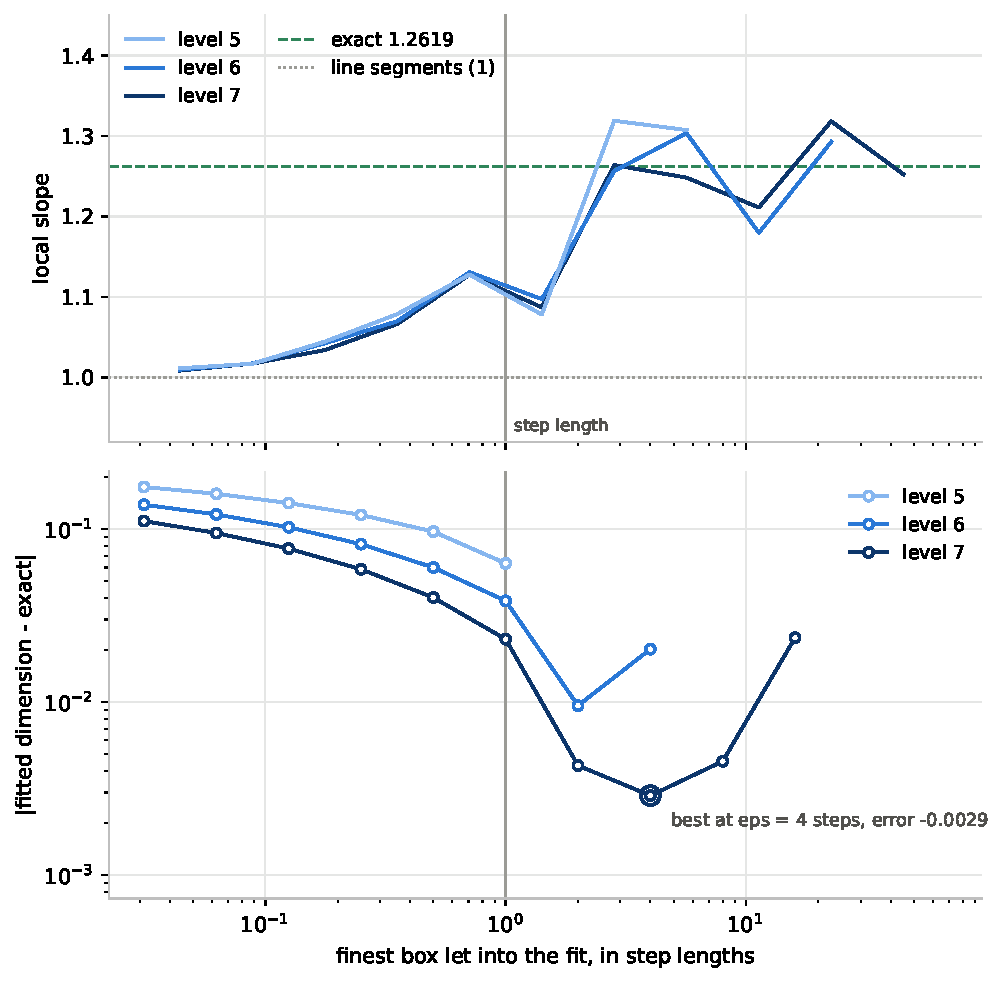
\includegraphics[width=\textwidth]{images/koch-rolloff.pdf}
    \caption{The Koch curve at levels 5--7. 
    \\\textbf{Top:} the local slope at
    each box size, near $\log4/\log3$ in the window and falling to 1 below the
    step length.  
    \\\textbf{Bottom:} the absolute error of a fit that starts at
    that box size, with the top end fixed. At level 7 the best start gives an
    error of $0.0029$; starting from the smallest box gives $0.1112$.
    Deeper levels move the V down and to the left.}
    \label{fig:rolloff}
\end{figure}

\begin{table}[H]
\centering
\begin{tabular}{rrrr}
\hline
$\eps_{\min}$ (steps) & points & fitted $\Bd$ & error \\
\hline
$1/32$ & 12 & $1.1507$ & $-0.1112$ \\
$1/8$  & 10 & $1.1848$ & $-0.0771$ \\
$1/2$  & 8  & $1.2217$ & $-0.0402$ \\
$1$    & 7  & $1.2388$ & $-0.0231$ \\
$2$    & 6  & $1.2576$ & $-0.0043$ \\
$4$    & 5  & $\mathbf{1.2590}$ & $\mathbf{-0.0029}$ \\
$8$    & 4  & $1.2664$ & $+0.0045$ \\
$16$   & 3  & $1.2854$ & $+0.0235$ \\
\hline
\end{tabular}
\caption{Koch at level 7, exact dimension $\log4/\log3=1.261860$. 
Each row fits the same coarse end and a different fine end.}
\label{tab:rolloff}
\end{table}

\noindent Hilbert shows the same thing with no noise at all (Figure~\ref{fig:rolloff-hilbert}). 
Fitting from $\ell$ gives exactly $2$, but each dyadic scale below it drags the answer towards $1$: $1.700$, then$1.500$, and $1.226$ by $\ell/32$. 
The estimator is not noisy, just wrong \texttt{:D}.

\begin{figure}[H]
    \centering
    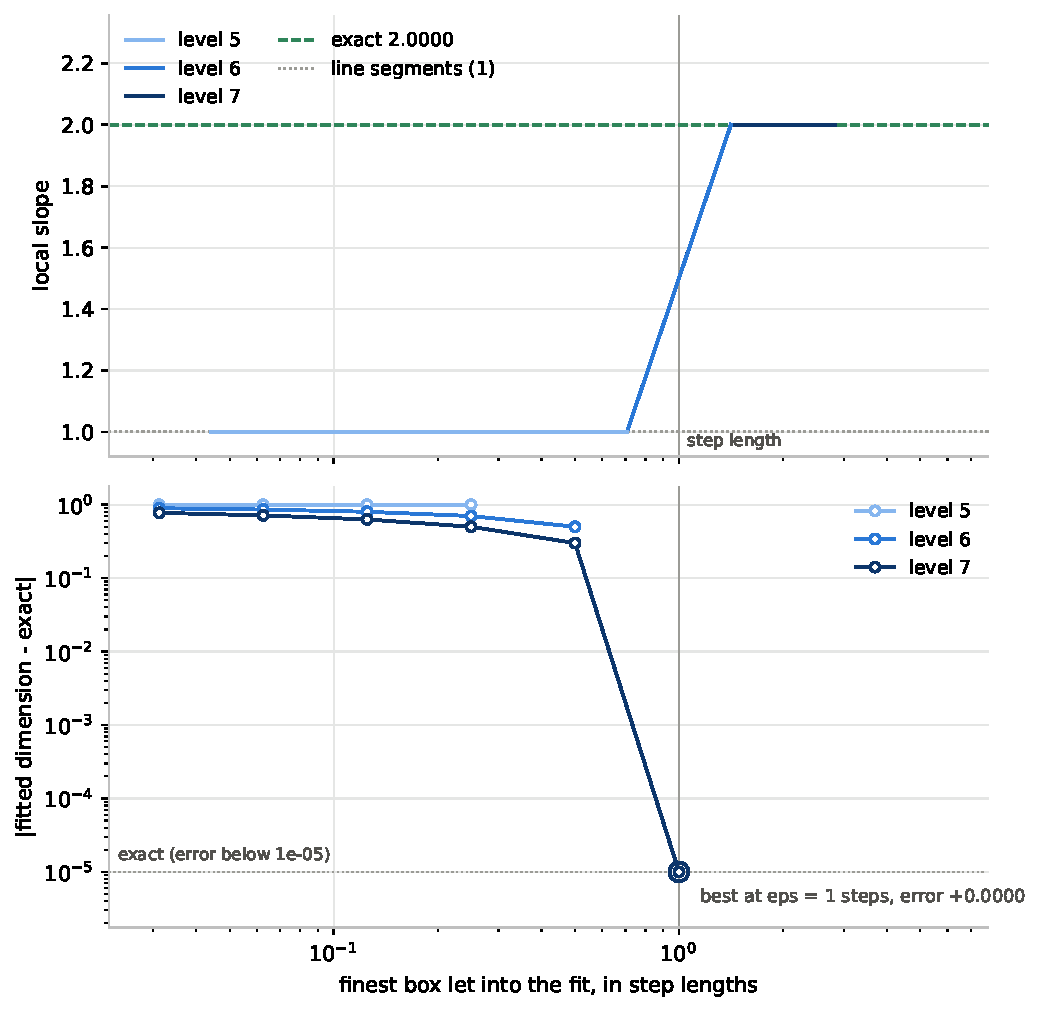
\includegraphics[width=\textwidth]{images/hilbert-rolloff.pdf}
    \caption{The same sweep on the Hilbert curve, levels 5--7.}
    \label{fig:rolloff-hilbert}
\end{figure}

\begin{remark}[The standard error]
\label{rem:errorbar}
    A standard error measures how far the points scatter around the fitted line, assuming the scatter is random. 
    However, here the points bend in one direction. 
    In the Koch example above, adding points below the step length made the standard error smaller and the estimate worse. 
    The spread of the local slopes says more about whether the plot is straight.
\end{remark}

\begin{remark}[The sign of the bias]
\label{rem:bias-sign}
    Box sizes below the step length pull the estimate towards $1$: down for
    Koch ($-0.0231$ starting at $\ell$, $-0.1112$ at $\ell/32$) but up for
    Cantor, with dimension $<1$ ($-0.0080$ at $\ell$, $+0.0254$ at $\ell/16$). 
    There's no fixed sign for fits starting with larger box sizes since it becomes the outline of the shape.
\end{remark}


% ─────────────────────────────────────────────────────────────────────────────
\newpage
\subsection{Final estimates}
\label{sec:estimates}

Table~\ref{tab:estimates} runs every system at the deepest level that traces in reasonable time. 
``Oct.'' is the width of the window in octaves, $\log_2(\operatorname{span}/32\ell)$; 
``pts'' is the number of box sizes in it;
and ``local slope'' is the range of $s(\eps)$ inside it.

\begin{table}[H]
\centering
\begin{tabular}{lrrrrlrrr}
\hline
system & $n$ & segments & oct. & pts & local slope & Mode A & Mode B & error \\
\hline
Cantor    & 14 & $16\,384$  & $17.2$ & 18 & $0.415$--$1.000$ & $0.630930$ & $0.6263$ & $-0.0047$ \\
Koch      &  8 & $65\,536$  & $7.7$  &  8 & $1.087$--$1.297$ & $1.261860$ & $1.2375$ & $-0.0243$ \\
Minkowski &  6 & $262\,144$ & $7.0$  &  8 & $1.307$--$1.564$ & $1.500000$ & $1.4687$ & $-0.0313$ \\
Arrowhead & 12 & $531\,441$ & $7.0$  &  8 & $1.337$--$1.601$ & $1.584963$ & $1.5525$ & $-0.0325$ \\
Peano     &  6 & $531\,441$ & $4.5$  &  5 & $1.969$--$1.992$ & $2.000000$ & $1.9783$ & $-0.0217$ \\
Hilbert   &  8 & $65\,535$  & $3.5$  &  4 & $2.000$--$2.000$ & $2.000000$ & $2.0000$ & $-0.0000$ \\
\hline
Gasket    & 10 & $177\,147$ & $5.0$  &  6 & $1.557$--$1.580$ & $1.584963$ & $1.5696$ & $-0.0154$ \\
Gosper    &  7 & $823\,543$ & $5.1$  &  6 & $1.928$--$1.992$ & $2.000000$ & $1.9683$ & $-0.0317$ \\
L\'evy C  & 16 & $65\,536$  & $4.0$  &  5 & $1.606$--$1.825$ & $2.000000$ & $1.7555$ & $-0.2445$ \\
Dragon    & 16 & $65\,536$  & $3.7$  &  4 & $1.762$--$1.819$ & $2.000000$ & $1.7835$ & $-0.2165$ \\
\hline
\end{tabular}
\caption{Mode B against the exact dimension; Mode A's error is zero on every row. 
The two that fail have $k=\sqrt2$ (\S\ref{sec:failures}).}
\label{tab:estimates}
\end{table}

\subsubsection{Why the last two fail}
\label{sec:failures}

Each level enlarges the figure by $k$, so the window grows by $\log_2 k$
octaves per level,
\[
  \log_2\!\frac{\operatorname{span}}{32\,\ell}
  \;=\; n\log_2k+\log_2C-5,
\]
which is $1.585$ for Koch but only $0.5$ for $k=\sqrt2$. The dragon at level 16
($65\,536$ segments) has $3.7$ octaves, about as much as Koch at level 5 or 6,
and matching Koch at level 8 would take level 24 ($1.7\times10^7$ segments).
This is why you can't just keep iterating to a deeper level. 
Also it is non-identifying since hilbert is exact but has a narrower window.

The local slopes do not identify them either. Starting at $2\ell$ to exclude the crossover
(Remark~\ref{rem:crossover}), with spread the largest minus the smallest and drift the last minus the first:
\[
\begin{array}{lrrr}
\hline
\text{system} & \text{local slopes},\ \eps\geq2\ell & \text{spread} & \text{drift}\\
\hline
\text{Koch (8)}      & 1.246\;1.245\;1.230\;1.297\;1.228\;1.265 & 0.069 & +0.019\\
\text{Arrowhead (12)}& 1.538\;1.557\;1.577\;1.591\;1.578\;1.601 & 0.063 & +0.063\\
\text{L\'evy C (16)} & 1.755\;1.825\;1.800                      & 0.070 & +0.045\\
\text{Dragon (16)}   & 1.762\;1.777                             & 0.015 & +0.015\\
\hline
\end{array}
\]
L\'evy C looks like Koch, and the Arrowhead drifts more than L\'evy C.
You can see that the dragon has the flattest slope but it's out by $0.22$.

\begin{remark}[Limits of the plateau]
\label{rem:plateau-limits}
    Local slopes that disagree means the plot is bending. Slopes that agree only suggest that it's straight, not necessarily correct.
    The dragon is off by the same amount each time so they agree on the wrong value!! With only 2 or 3 points a local slope can't really tell you anything sometimes.
\end{remark}

\noindent  L\'evy C keeps improving up to the coarsest start at level 16 ($-0.2445$ at $\ell$, $-0.2032$ at $2\ell$,$-0.1871$ at $4\ell$).
This means that the bottom of the V is not in reach and we just need to iterate more levels. The dragon has no such pattern you can use.

\subsubsection{The settling test}
\label{sec:levels}

We can attempt to find failures by running the estimate at several levels and checking whether it has stopped moving. 
We don't want to tune after the fact (Remark~\ref{rem:nocheat}) since it is ``cheating'' so the test is fixed in advance:

\begin{quote}\small
Take three levels $n_0<n_1<n_2$ that differ in size by at least a factor of 2
($k^{n_{i+1}-n_i}\geq2$: adjacent levels for $k\geq2$, every second level for
$k=\sqrt2$), each with at least two box sizes in its window. Let $\hat D_i$ be
the Mode B estimate at level $n_i$, and write
\[
  m_1=|\hat D_1-\hat D_0|,\qquad m_2=|\hat D_2-\hat D_1|
\]
for the two moves between them. With $p$ the placement spread at the deepest
level (Remark~\ref{rem:offsets}), the estimate is \textbf{still moving} if
$m_2>\max(\tau,p)$, \textbf{settled} if $m_2\leq\tau$, and
\textbf{indeterminate} in between. Here $\tau=0.005$.
\end{quote}

\noindent The levels must differ by at least a factor of 2 so that we can measure at least one more box width (i.e. for Dragon this is every 2 levels since $k=\sqrt2$). 
The test uses $m_2$ rather than the ratio $m_2/m_1$ since we're looking at convergence ($m_1$ is mostly just for context).
The $p$ term stops a move that could be due to grid placement from counting as a change with level (uncertainty).
All estimates are taken on the unshifted grid, so ``settled'' means settled at that one placement.

\begin{table}[H]
\centering
\begin{tabular}{llrrrlr}
\hline
system & levels & $m_1$ & $m_2$ & $p$ & verdict & $|$error$|$ \\
\hline
Hilbert   & 6/7/8    & $0.0000$ & $0.0000$ & $0.029$ & settled & $0.0000$ \\
Koch      & 6/7/8    & $0.0153$ & $0.0013$ & $0.007$ & settled & $0.0243$ \\
Gasket    & 8/9/10   & $0.0033$ & $0.0015$ & $0.030$ & settled & $0.0154$ \\
Peano     & 4/5/6    & $0.0444$ & $0.0018$ & $0.012$ & settled & $0.0217$ \\
Gosper    & 5/6/7    & $0.0224$ & $0.0019$ & $0.001$ & settled & $0.0317$ \\
Cantor    & 12/13/14 & $0.0016$ & $0.0026$ & $0.018$ & settled & $0.0047$ \\
\hline
Minkowski & 4/5/6    & $0.0444$ & $0.0199$ & $0.025$ & \emph{indeterminate} & $0.0313$ \\
\hline
Arrowhead & 10/11/12 & $0.0071$ & $0.0255$ & $0.004$ & \textbf{still moving} & $0.0325$ \\
Dragon    & 12/14/16 & $0.0575$ & $0.0562$ & $0.032$ & \textbf{still moving} & $0.2165$ \\
L\'evy C  & 12/14/16 & $0.1145$ & $0.0677$ & $0.056$ & \textbf{still moving} & $0.2445$ \\
\hline
\end{tabular}
\caption{The settling test on all ten systems.}
\label{tab:levels}
\end{table}

\noindent Four things follow from the table.
\begin{itemize}
    \item \textbf{Choice of $\tau$.} No system has $m_2$ between Cantor's
    $0.0026$ and Minkowski's $0.0199$, so any $\tau$ in that range gives the same table.
    \item \textbf{Settled doesn't imply correctness.} Gosper settles ($m_2=0.0019$) but is still out by $0.0317$. This just means that deeper levels won't help.
    \item \textbf{Not settled doesn't imply incorrectness.} 
    The Arrowhead is flagged although it is within $0.033$ since it's estimate is moving by $0.0255$ between levels 11 and 12. This means that level 13 would get more information.
    \item \textbf{Cost.} Shallower levels together cost $\lambda^{-1}+\lambda^{-2}$ times level $n$ for a max of $0.75\times$ extra (at $\lambda=2$).
\end{itemize}

\subsubsection{Choosing the floor}
\label{sec:floor}

The floor is the smallest box size the fit uses. Table~\ref{tab:floor} compares a floor of $\ell$ with one of $2\ell$.

\begin{table}[H]
\centering
\begin{tabular}{lrrrrr}
\hline
 & & \multicolumn{2}{c}{floor at $\ell$} & \multicolumn{2}{c}{floor at $2\ell$} \\
system & $n$ & pts & error & pts & error \\
\hline
Cantor    & 14 & 18 & $-0.0047$ & 17 & $-0.0072$ \\
Koch      &  8 &  8 & $-0.0243$ &  7 & $\mathbf{-0.0099}$ \\
Minkowski &  6 &  8 & $-0.0313$ &  7 & $-0.0147$ \\
Arrowhead & 12 &  8 & $-0.0325$ &  7 & $\mathbf{-0.0100}$ \\
Peano     &  6 &  5 & $-0.0217$ &  4 & $-0.0263$ \\
Hilbert   &  8 &  4 & $-0.0000$ &  3 & $+0.0000$ \\
Gasket    & 10 &  6 & $-0.0154$ &  5 & $-0.0169$ \\
Gosper    &  7 &  6 & $-0.0317$ &  5 & $-0.0387$ \\
L\'evy C  & 16 &  5 & $-0.2445$ &  4 & $-0.2032$ \\
Dragon    & 16 &  4 & $-0.2165$ &  3 & $-0.2305$ \\
\hline
\end{tabular}
\caption{Raising the floor from $\ell$ to $2\ell$. Bold means the difference is larger than $p$.}
\label{tab:floor}
\end{table}

\noindent Dropping the smallest box size helps when enough points are left:
Koch, Minkowski and the Arrowhead (seven left) improve $2-3\times$, while
the Gasket, Gosper and Peano (five or fewer) get worse. Cantor gets worse even
with 17 points because its dimension is below 1 (Remark~\ref{rem:bias-sign}). 
I figure that a potential rule could be: \emph{start at $2\ell$ if at least six points remain, otherwise at $\ell$.} 
Its average error over the eight working systems is $0.0138$, against $0.0202$ starting at $\ell$ and $0.0155$
at $2\ell$, but with an uncertainty of about $0.0034$ these are too close to rank (only Koch and Arrowhead clearly benefit (see Table \ref{tab:floor})).

\begin{remark}[``Cheating'']
\label{rem:nocheat}
    Dropping the smallest box size follows from the crossover (Remark~\ref{rem:crossover}), but the threshold of six was picked by looking at the computed number compared to the actual number (what we're trying to find).
    So Table~\ref{tab:estimates} still starts at $\ell$: you can't test on a rule you get from looking at the error since it is cheating (circular reasoning).
\end{remark}


% ─────────────────────────────────────────────────────────────────────────────
\subsection{What each mode is good for}

Mode A is exact on every system, including when $k$ is measured. 
Mode B is within $0.034$ on eight of the ten, but out by more than $0.21$ on the other two without a method of distuinguishing correctness.
However, only Mode B can be run on a coastline, so a box-counting dimension should be reported with, in order of usefulness:

\begin{enumerate}
    \item \textbf{the estimate at two or three levels}, with the settling test (\S\ref{sec:levels});
    \item \textbf{the placement spread} (Remark~\ref{rem:offsets}), $0.001$ to $0.056$ here, as large as the errors themselves;
    \item \textbf{the level and the window} (confidence);
    \item \textbf{the spread of the local slope}, curvature check (Remark~\ref{rem:plateau-limits}).
\end{enumerate}

\noindent Running \texttt{boxcount} prints this (\texttt{--settle }flag for settling test).

% ─────────────────────────────────────────────────────────────────────────────
\subsection{Improvements}
\label{sec:improvements}

\begin{itemize}
    \item \textbf{A system whose $k$ needs the diameter.} 
    No system in the library needs the diameter fallback of Remark~\ref{rem:endpoint}, so that route has never been used for an answer. 
    Need a system that has a displacement that doesn't grow and also that you can't walk the production.
    I could add the Moore curve, a closed loop of four Hilbert curves, which I believe would need it.

    \item \textbf{Rotating calipers.} 
    The diameter of a convex polygon with $h$ vertices can be found in $O(h)$ by rotating calipers, instead of the $O(h^2)$ blocked search over all pairs. 
    This makes no difference to our library which has hulls of max 10 points, but if the hull was very large such as a point cloud it would be a useful improvement.

    \item \textbf{Exact coordinates at $60^\circ$ and $45^\circ$.} Storing positions as integer combinations of the turn angle's step directions would make the unshifted grid's tie-breaks exact for every system.
    However, I'd still need a fallback for arbitrary angles.

    \item \textbf{More placements.} Three random grids give only a rough spread. 
    With more, the mean over placements could replace the unshifted grid as the reported number (Remark~\ref{rem:offsets}).
    This is an expensive operation, hwoever.

    \item \textbf{A floor found from the data.} Mode B's floor is the step length $\ell$, which a photograph does not come with. 
    It could instead be detected as the box size where the local slope leaves 1.

    \item \textbf{Testing the rules on new systems.} The floor threshold was fitted on this family.
    I should probably validate these with a new set...
\end{itemize}


% ─────────────────────────────────────────────────────────────────────────────
\newpage
\printbibliography
% ─────────────────────────────────────────────────────────────────────────────

\end{document}